% Audited revision, 2026-09-04. Original ACC2027_v4.tex is preserved.
% Working IEEE two-column layout. Apply the official ACC author kit before
% submission; the installed IEEEconf class is NOT the PaperPlaza ieeeconf.
\documentclass[letterpaper,10pt,conference]{IEEEtran}
\usepackage{amsmath,amssymb,amsthm,bm}
\usepackage{booktabs,array,cite}
\usepackage{graphicx}
\usepackage[hidelinks]{hyperref}
% Figures live under figures/..., so keep that on the graphics path.
\graphicspath{{figures/}{../experiments/nengo_nef_replication_2026-08-29/results/plots/}}


\newcommand{\R}{\mathbb R}
\newcommand{\T}{^{\mathsf T}}
\newcommand{\sat}{\operatorname{sat}}
\newcommand{\clip}{\operatorname{clip}}
\newcommand{\sgnp}{\operatorname{sgn}_{+}}
\newtheorem{proposition}{Proposition}
\newtheorem{remark}{Remark}

\title{Online PES-Adapted Neuromorphic Membrane--Gate Residual Control for
Actuator-Constrained UAV Quaternion Attitude Tracking}
\author{%
\IEEEauthorblockN{Gandhi Contreras\IEEEauthorrefmark{1}, Steven Sandoval\IEEEauthorrefmark{1}, Luis Garcia\IEEEauthorrefmark{2}}%
\IEEEauthorblockA{\IEEEauthorrefmark{1}New Mexico State University (NMSU), Las Cruces, NM, USA}%
\IEEEauthorblockA{\IEEEauthorrefmark{2}U.S. Air Force, Los Alamos, NM, USA}%
}

\begin{document}
\maketitle
\thispagestyle{empty}
\pagestyle{empty}

\begin{abstract}
We study a compact neuromorphic residual architecture for quaternion attitude
tracking with bounded actuator commands. A fixed quaternion proportional--
derivative (PD) controller is augmented by six paired continuous
coupled membrane--gate (CMG) units whose gate-derived activities are decoded
through eighteen weights adapted online by prescribed error sensitivity
(PES). We distinguish intrinsic conductance modulation, decoder learning,
and residual authority, and establish bounded neural states, bounded command
deviation, projected decoder boundedness, and a restricted frozen-feature
learning result. These properties do not imply closed-loop stability or
saturation-free rotor allocation. In ten matched 45-s MuJoCo cases spanning
five missions, a Skydio X2 model and a Crazyflie~2.0 (CF2) model with an
explicit four-rotor actuation extension exhibit 17.3--60.6\% lower mean
quaternion-angle error than PD. Actuator-bound occupancy is zero except for
brief Hardstep intervals. Direct and Nengo realizations agree within
$2.013\times10^{-6}$ in relative mean-error difference. Ablations identify
online decoder adaptation, rather than conductance modulation, as the
principal source of improvement in the tested amplified-gate regime. An
annealed activity-trace learning variant is examined separately in the
precursor architecture, with both beneficial and adverse outcomes.
Preliminary physical 3DOF Hover Roll tests provide supporting evidence: three
matched pairs improve their recorded mean error by
$2.65\%\pm1.08\%$ (sample standard deviation).
\end{abstract}

\section{Introduction}
Learning-based augmentation can retain useful classical feedback structure
while adapting a correction that is difficult to specify a priori.
Residual robot control is established \cite{johannink2019}; quadrotor
examples include geometric $\mathcal L_1$ augmentation with performance
guarantees \cite{wu2025l1quad} and PID-plus-PPO attitude residuals
\cite{li2027hpappo}. Thus, neither additive residual learning nor online
flight adaptation is novel in isolation.

Neuromorphic control offers a complementary implementation approach.
Nengo supports the Neural Engineering Framework (NEF) and online decoder
learning \cite{bekolay2014nengo}. PES-based adaptive control has been
demonstrated on manipulators \cite{dewolf2016arm,dewolf2020nengo}, and a
Nengo spiking PID controller with PES-based self-tuning has been validated
on a free-flying UAV \cite{olivares2026selftuning}. Our contribution is not
the first PES/Nengo UAV controller. Instead, we investigate a specific
continuous membrane--gate basis for a bounded quaternion-torque residual,
with a fixed classical controller and adaptation confined to its decoder.

The central question is whether this small stateful basis can improve
tracking, and which of its components explains the improvement. The paper
contributes: (i) a code-aligned CMG--PES architecture with paired currents,
explicit state/readout equations, and actuator interfaces; (ii) precise
boundedness and baseline-recovery properties, without an unsupported
closed-loop stability claim; (iii) a five-mission, two-model study with
direct/Nengo agreement and neuron-family comparisons; and (iv) a separate
study of annealed activity-trace learning that documents its implementation
and evidence limitations. Selected preliminary Hover tests support
physical feasibility but are not the main validation claim.

Here ``neuromorphic'' refers to neuron-inspired continuous state dynamics,
local error-directed learning, and a neural-simulator realization. The
implementation does not emit spikes and has not been deployed on
neuromorphic hardware; no power advantage is claimed. PES is an
established rule, and novelty is claimed for its integration and controlled
evaluation in this architecture, not for PES itself.

\begin{figure}[!h]
\centering
\includegraphics[width=\linewidth]{\detokenize{all/skydio_crazyflie_models_cropped (1)}}
\caption{Skydio X2 (X2) and Crazyflie~2.0 (CF2) MuJoCo model geometries. The shown axis triads are body-frame axes; they are rigidly attached to the vehicle and therefore rotate with the vehicle relative to the inertial (world) frame (cf. $Q\!:\,\text{body}\to\text{inertial}$ in Sec.~\ref{sec:problem}).}
\label{fig:scale}
\end{figure}

\begin{figure*}[t]
\centering
\begin{minipage}[t]{0.48\textwidth}\centering
\includegraphics[width=\linewidth]{\detokenize{all/crazyflie2_cropped (1)}}
\end{minipage}\hfill
\begin{minipage}[t]{0.48\textwidth}\centering
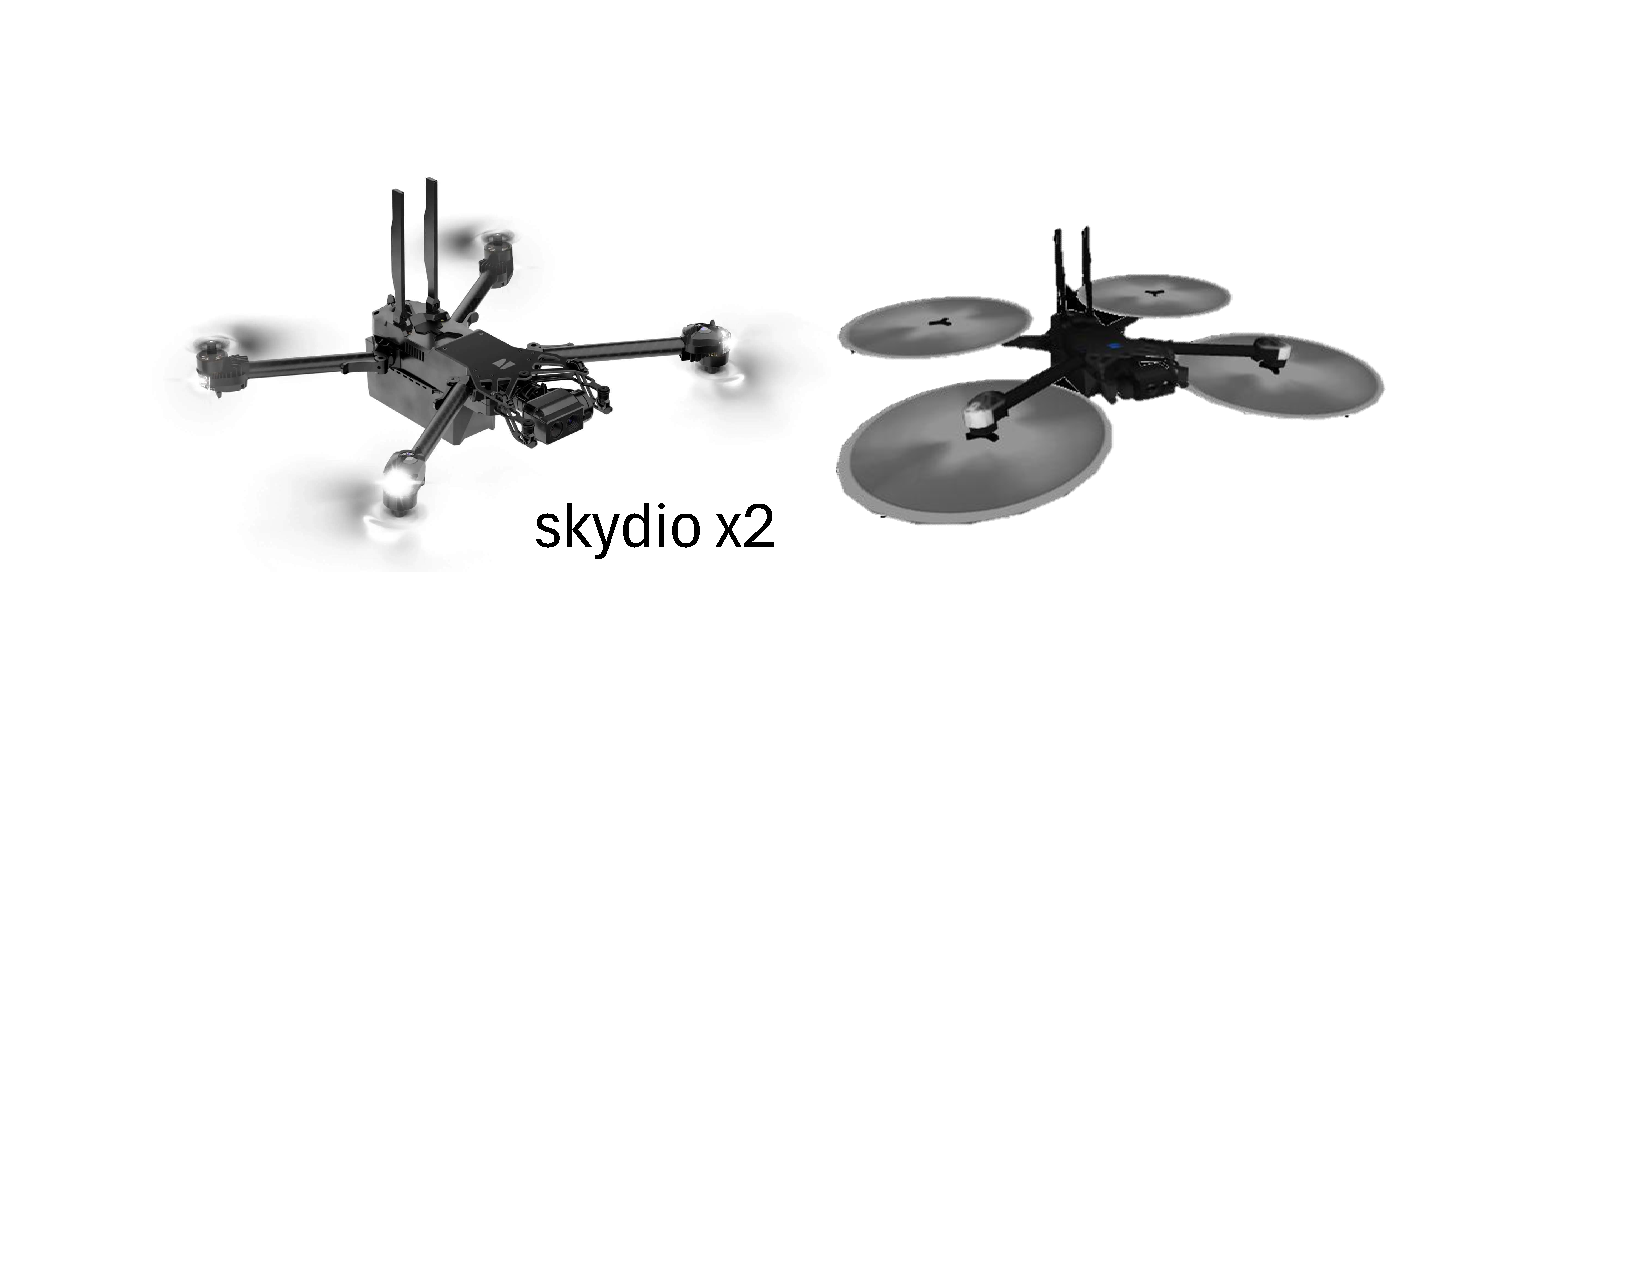
\includegraphics[width=\linewidth]{all/skydiox2_cropped}
\end{minipage}
\caption{Hardware-Drones and MuJoCo model geometries used in simulation: CF2 (left) and X2 (right).}
\label{fig:models}
\end{figure*}


%%%%%%%%%%%%%%%%%%%%%%%%%%%%%%%%%%%%%%%%%%%%%%%%%%%%%%%%%%%%%%%%%%%%%%%%%%
\section{Simulation Models, Attitude Baseline, and Actuator Interface}
\label{sec:problem}
%%%%%%%%%%%%%%%%%%%%%%%%%%%%%%%%%%%%%%%%%%%%%%%%%%%%%%%%%%%%%%%%%%%%%%%%

\subsection{MuJoCo Platforms and CF2 Actuation Extension}
We use Crazyflie 2.0 (CF2) and Skydio X2 (X2) models derived from MuJoCo
Menagerie \cite{menagerieModels}. Each vehicle has six rigid-body degrees of freedom: three
translations and three rotations, represented by seven free-joint position
coordinates (position and unit quaternion) and six velocity coordinates.
The attitude controller requests three body torques; a separate classical
height loop requests collective thrust. Thus attitude tracking is evaluated
in a freely translating model, not an attitude-only joint model.

The upstream CF2 interface provides collective thrust and three abstract
body-moment channels; its documentation identifies the original actuator
limits as arbitrary and requiring tuning \cite{menagerieCF2}. Our four-rotor actuation extension replaces that
interface with four nonnegative, spatially located thrust inputs while
retaining the source mass, inertia, and visual geometry. Rotor moment arms
and signed reaction-torque coefficients define an explicit allocation
matrix, making the coupling between collective thrust, attitude torque,
and individual actuator limits testable. This is a model-interface
contribution, not a complete aerodynamic identification of CF2.

\begin{table}[!ht]
\centering
\caption{Compiled simulation-model characteristics. CF2 authority is
scaled relative to the upstream model limit, not a manufacturer rating.
Hardware comparisons are given in Table~\ref{tab:manufacturer}.}
\label{tab:models}
\setlength{\tabcolsep}{3pt}
\footnotesize
\begin{tabular}{@{}p{0.40\linewidth}p{0.27\linewidth}p{0.25\linewidth}@{}}
\toprule
Property & CF2 rotor model & X2 model\\
\midrule
Mass $M$ (kg) & $0.027$ & $1.325$\\
Rotor $|p_x|,|p_y|$ (m) & $0.0325,0.0325$ & $0.14,0.18$\\
Reaction magnitude $|\kappa_i|$ (m) & $0.005$ & $0.0201$\\
Unscaled rotor limit (N) & $0.0875$ & $13$\\
Main-test authority scale & $1.5$ & $1$\\
Main-test rotor limit (N) & $0.13125$ & $13$\\
Main-test total limit (N) & $0.525$ & $52$\\
Maximum thrust/weight & $1.321\to1.982$ & $4.001$\\
Rigid-body integrator & RK4 & Euler\\
Experiment timestep (s) & $0.0005$ & $0.0005$\\
Motor activation/RPM states & None & None\\
\bottomrule
\end{tabular}
\end{table}

For CF2, the unscaled model's total thrust limit is $0.35$ N. We evaluate
a rotor-interface model with increased actuator authority: multiplying
$f_{\max,i}$ by $1.5$ yields $0.525$ N total
(Table~\ref{tab:models}). This raises the modeled maximum thrust/weight
from $1.321$ to $1.982$ at $g=9.81$ m/s$^2$. For physical perspective,
constant-height flight at a single-axis $45^\circ$ tilt requires
$T/(Mg)=1/\cos45^\circ=\sqrt{2}$ even before reserving differential-thrust
margin. The unscaled model cannot meet that idealized requirement; this
does not establish such a limitation for stock CF2 hardware. The scale
changes a simulation thrust bound, not rotor speed, stock propulsion
capability, or tracking performance by $50\%$. Mass, inertia, and reaction
coefficients are unchanged. PD and CMG use the same model and actuator
bounds; any benefit from increased model authority is therefore distinct
from the benefit of neural augmentation.

\begin{table}[!ht]
\centering
\caption{Simulation parameters versus manufacturer information.
``Not reported'' refers to the manufacturer sources reviewed, not proof
that the parameter is unavailable elsewhere.}
\label{tab:manufacturer}
\setlength{\tabcolsep}{3pt}
\footnotesize
\begin{tabular}{@{}>{\raggedright\arraybackslash}p{0.25\linewidth}>{\raggedright\arraybackslash}p{0.30\linewidth}>{\raggedright\arraybackslash}p{0.37\linewidth}@{}}
\toprule
Quantity & Simulation & Manufacturer information\\
\midrule
CF2 mass & $27$ g & $27$ g \cite{bitcrazeCF20Specs}\\
X2 mass & $1325$ g & $1325$ g with battery \cite{skydioX2ESpecs}\\
CF2 total thrust & $0.350\to0.525$ N & $0.568$ N measured at $93.75\%$ PWM\textsuperscript{a} \cite{bitcrazeThrustMeasurements}\\
X2 rotor limit & $13$ N per rotor & Not reported \cite{skydioX2ESpecs}\\
CF2 motor response & No motor dynamics & $\sim180$ ms: $0\to25{,}000$ RPM\textsuperscript{b} \cite{bitcrazeMotorResponse}\\
Inertia tensors & CF2 inherited; X2 geometry-derived & Not reported in product specifications \cite{bitcrazeCF20Specs,skydioX2ESpecs}\\
\bottomrule
\end{tabular}
\par\smallskip
\begin{minipage}{0.97\linewidth}
\scriptsize
\textsuperscript{a}Historical total-thrust measurement with a power-supply
test setup, not a guaranteed continuous battery-powered rating.
\textsuperscript{b}One motor's reported full-command response with a
charged battery; not an identified first-order time constant.
\end{minipage}
\end{table}

The masses agree with published specifications, but this does not
validate all dynamic parameters (Table~\ref{tab:manufacturer}). Bitcraze's
historical measurement of $57.9$ gram-force corresponds to approximately
$0.568$ N; the evaluated $0.525$ N limit is about $7.5\%$ below that
operating point \cite{bitcrazeThrustMeasurements}. This supports a plausible
thrust scale, not hardware validation, and does not establish that a
stronger-than-stock motor is required. CF2 inertia is inherited from
Menagerie, which cites system-identification work \cite{menagerieCF2}; the
rotor-extension moment arms and $|\kappa_i|=0.005$ m remain design
assumptions. X2 inertia, $13$ N rotor limits, and $|\kappa_i|=0.0201$ m are
simulation parameters, not confirmed manufacturer characteristics.

Geometric dimensions also require like-for-like definitions. Bitcraze
lists $92\times92\times29$ mm motor-to-motor/height dimensions
\cite{bitcrazeCF20Specs}; our sites give an opposite-motor separation of
$91.92$ mm. Skydio lists an unfolded flying envelope of approximately
$663\times569\times211$ mm \cite{skydioX2ESpecs}, whereas the model's rotor
centers span $280\times360$ mm. Center spacing and overall flying envelope
are different quantities and do not by themselves establish geometric
agreement or mismatch. Propulsion identification, motor and battery
dynamics, and experimental validation remain necessary for hardware
transfer; no endurance or electrical-power fidelity is claimed.

MuJoCo \cite{todorov2012mujoco} integrates rigid-body motion, gravity, site-applied actuator
wrenches, and enabled passive/contact forces. Both models specify air
density $1.225$ kg/m$^3$ and viscosity $1.8\times10^{-5}$ Pa\,s; their
default inertia-based fluid model \cite{mujocoFluid} is a coarse drag approximation, not
rotor-resolved aerodynamics. The runner overrides the timestep but retains
each model's integrator. Actuators apply algebraic thrust commands without
motor activation dynamics. Although gyro, accelerometer, and orientation
sensors are defined, the evaluated feedback is read directly from
\texttt{qpos}/\texttt{qvel}; optional measurement perturbations are separate
runner settings. These experiments do not establish performance with a
hardware state estimator.

%\input{figure1_interface.tex}

\subsection{Quaternion Convention and Error}
Let $Q\in\mathbb S^3$ be the scalar-first Hamilton quaternion mapping body
coordinates to inertial coordinates, and let $\bm\omega$ be body angular
velocity. With physical inertia $\bm J\succ0$ about the center of mass,
expressed in body axes, the free-flight rotational balance is
\begin{align}
 \dot Q&=\tfrac12 Q\otimes[0,\bm\omega\T]\T,\\
 \bm J\dot{\bm\omega}&=\bm\tau_{\rm act}+\bm\tau_{\rm p}
       +\bm\tau_{\rm d}-\bm\omega\times(\bm J\bm\omega).
 \label{eq:plant}
\end{align}
Here $\bm\tau_{\rm p}$ denotes modeled passive torque and
$\bm\tau_{\rm d}$ any applied disturbance; the nominal ideal rigid-body
model sets both to zero. Contact, if present, contributes an additional
external wrench. The requested torque and actuator torque are distinct
signals in Fig.~\ref{fig:scale}.

The controller conjugates MuJoCo's orientation and uses the passive
quaternion $q=Q^{-1}$, so
\begin{equation}
 \dot q=-\tfrac12[0,\bm\omega\T]\T\otimes q.
 \label{eq:passive}
\end{equation}
The desired $q_d$ uses the same convention. Define
\begin{align}
 q_e&=q_d\otimes q^{-1}=[q_{e,0},\bm q_{e,v}\T]\T,\\
 \bm e_q&=\sgnp(q_{e,0})\bm q_{e,v},\qquad \sgnp(0)=1,\\
 \theta_q&=2\operatorname{atan2}(\|\bm q_{e,v}\|_2,|q_{e,0}|)
             \in[0,\pi].
 \label{eq:theta}
\end{align}
The reported error $\theta_q$ is the shortest rotation angle, invariant
under $q_e\mapsto-q_e$. Sign selection introduces a discontinuity at
$q_{e,0}=0$; it does not establish robust hybrid global stability
\cite{mayhew2011hybrid}.
For a desired-frame rate $\bm\omega_d$ satisfying the corresponding
passive kinematics, differentiation gives
\begin{align}
 \dot q_e&=\tfrac12q_e\otimes[0,\bm\omega_e\T]\T,\\
 \bm\omega_e&=\bm\omega-R(q_e)\T\bm\omega_d,\qquad
 \dot q_{e,0}=-\tfrac12\bm q_{e,v}\T\bm\omega_e.
 \label{eq:errkin}
\end{align}
This is a kinematic identity, not a convergence result. Reference Euler
triples parameterize $q_d$ in the passive convention, rather than active
body-to-world Euler commands.

\subsection{Physical Inertia and Implemented PD Gains}
MuJoCo stores principal moments $\bm j_{\rm p}$ in its inertial frame
\cite{mujocoInertial}.
If $R_{BI}$ maps that frame into body axes, the physical inertia is
\begin{equation}
 \bm J=R_{BI}\operatorname{diag}(\bm j_{\rm p})R_{BI}\T.
 \label{eq:inertiaframe}
\end{equation}
The evaluated implementation uses a tuning vector
$\bm j_{\rm tune}=\bm j_{\rm p}$ directly, in the returned array order:
\begin{align*}
 \bm j_{\rm tune}^{\rm CF2}&=(2.3951,2.3951,3.2347)\T10^{-5},\\
 \bm j_{\rm tune}^{\rm X2}&=(0.0607113,0.0364684,0.0254117)\T,
\end{align*}
in kg\,m$^2$. CF2's inertial axes coincide with its body axes. For X2
they do not; its physical body-frame tensor is approximately
\begin{equation}
 \bm J_{\rm X2}=\begin{bmatrix}
 0.0366517&0&-0.0021000\\
 0&0.0254117&0\\
 -0.0021000&0&0.0605280
 \end{bmatrix}\ \mathrm{kg\,m^2}.
\end{equation}
Thus the tuning vector must not be identified with
$\operatorname{diag}(\bm J)$ for both vehicles.

The fixed quaternion PD baseline is
\begin{align}
 \bm k_q&=2\bm j_{\rm tune}\odot\bm\omega_n^2,\qquad
 \bm k_\omega=2\zeta\bm j_{\rm tune}\odot\bm\omega_n,\\
 \bm u_0&=\sat_{\bm\ell}
       (-\bm k_q\odot\bm e_q-\bm k_\omega\odot\bm\omega),
 \label{eq:pd}
\end{align}
where $\odot$ denotes componentwise multiplication,
$\bm\omega_n=(4,4,3.5)\T$ rad/s, $\zeta=0.95$, and
$\sat_{\bm\ell}$ clips component $i$ to $[-\ell_i,\ell_i]$.
For these rotor-interface models, the model-policy torque limits are
$\ell_i=\max(j_{{\rm tune},i}a_i,10^{-6}\ \mathrm{N\,m})$,
with $\bm a=(12,12,10)\T$ rad/s$^2$.
These are controller torque bounds, not guaranteed feasible rotor torques.
The law is quaternion feedback \cite{fresk2013quaternion};
$\bm\omega_n$ parameterizes its gains but is not a verified set of
closed-loop natural frequencies for coupled X2 dynamics.
Desired-rate feedforward and gyroscopic cancellation are omitted.
The identical fixed gains are retained for PD and its CMG augmentation.

For perspective only, take a constant reference, scalar proportional
gain $\bm k_q=k_q\bm1$, the ideal plant
($\bm\tau_{\rm p}=\bm\tau_{\rm d}=0$), no saturation or residual, and a
trajectory confined to one smooth sign branch. Then
$V=\frac12\bm\omega\T\bm J\bm\omega+2k_q(1-|q_{e,0}|)$ gives
$\dot V=-\bm\omega\T\operatorname{diag}(\bm k_\omega)\bm\omega$.
This restricted identity does not prove stability of the anisotropic,
saturated, moving-reference experiments.

\subsection{Requested and Realized Wrench}
For rotor positions $\bm p_i$ in body coordinates, parallel $+z$ thrust
axes, and signed reaction coefficients $\kappa_i$, define
\begin{equation}
 B=\begin{bmatrix}
 1&1&1&1\\p_{1,y}&p_{2,y}&p_{3,y}&p_{4,y}\\
 -p_{1,x}&-p_{2,x}&-p_{3,x}&-p_{4,x}\\
 \kappa_1&\kappa_2&\kappa_3&\kappa_4
 \end{bmatrix}.
 \label{eq:allocationmatrix}
\end{equation}
The signs follow $\bm p_i\times[0,0,f_i]\T$ and the actuator's local
reaction torque $\kappa_i f_i$. Both models have zero body-frame
center-of-mass $x,y$ offsets, so the site's $x,y$ coordinates also give
the relevant center-of-mass moment arms. Figure~\ref{fig:scale} fixes the
rotor ordering used by $B$; $\kappa_i$ has units of meters, not angular
velocity. The runner computes
\begin{equation}
 \begin{aligned}
 \bm f_{\rm req}&=B^{-1}[T,\bm u\T]\T,\\
 \bm f_{\rm act}&=\clip_{[\bm0,\bm f_{\max}]}(\bm f_{\rm req}),\\
 [T_{\rm act},\bm\tau_{\rm act}\T]\T&=B\bm f_{\rm act}.
 \end{aligned}
 \label{eq:mixer}
\end{equation}
Here $\bm u=\bm u_0$ for PD; the CMG path in Section~\ref{sec:architecture}
modifies that requested torque before the same allocation and clipping.
Each $f_i$ is a commanded force in newtons, not a rotor-speed command.
Exact wrench realization requires
$B^{-1}[T,\bm u\T]\T\in[\bm0,\bm f_{\max}]$.
A componentwise torque box is not generally contained in this
collective-dependent feasible set. Clipped inverse allocation is used,
not an optimization-based allocator \cite{monteiro2016allocation}.

Collective thrust remains classical, with $z_d=1$ m:
\begin{equation}
 T=\clip_{[0,2.5Mg]}
 \left(\frac{M[g+6(z_d-z)-4\dot z]}{\max(R(Q)_{33},0.35)}\right).
 \label{eq:collective}
\end{equation}
This expression uses the model's $g=9.81$ m/s$^2$. The height loop reads
free-joint height and vertical velocity; the denominator compensates tilt
with a lower guard. Its upper bound does not supersede individual rotor
limits. The CMG path has no direct collective output, but can affect
height through attitude, tilt compensation, and allocation saturation.
The resulting shared plant interface isolates changes in requested
attitude torque while preserving the same physical simulation for both
controllers.

%%%%%%%%%%%%%%%%%%%%%%%%%%%%%%%%%%%%%%%%%%%%%%%%%%%%%%%%%%%%%%%%%
\section{CMG State Dynamics and Online Decoder Adaptation}
\label{sec:architecture}
%%%%%%%%%%%%%%%%%%%%%%%%%%%%%%%%%%%%%%%%%%%%%%%%%%%%%%%%%%%%%%%%%
\subsection{Encoding, States, and Numerical Update}
For $m$ torque channels and $2m$ units, normalize the clipped baseline and
form positive/negative current pairs:
\begin{equation}
 \begin{aligned}
 \bar{\bm u}&=\bm u_0\oslash\bm\ell,\\
 \bm I^{\pm}&=I_b\bm1+I_g\max(\pm\bar{\bm u},\bm0),\\
 \bm I&=[(\bm I^+)\T,(\bm I^-)\T]\T.
 \end{aligned}
 \label{eq:encoding}
\end{equation}
Each unit has a dimensionless membrane state $v_j$ and gate $r_j$:
\begin{align}
 \dot r_j&=[\sigma(\alpha_h(v_j-v_{\rm th}+\gamma r_j))-r_j]/\tau_r,\\
 \dot v_j&=-(v_j-v_{\rm rest})/\tau+I_j/\tau-c_j(v_j-v_{\rm reset}),\\
 c_j&=(g_0+\chi g_1|I_j|)r_j^2,\qquad \chi\in\{0,1\}.
 \label{eq:cmg}
\end{align}
The logistic gate target depends on $v_j$, while $r_j$ shifts that target
and modulates membrane conductance. Thus, both states participate even
though the decoder reads the gate-derived activity. The model has no
threshold-triggered reset or spike event; $v_{\rm reset}$ is a reversal
level in a continuous conductance term. The gains $g_0,g_1$ have the units
needed to make $c_j$ a rate.

The actual integration is sequential, not exponential Euler for both
states. From the old states compute
\begin{align}
 b_{j,k}&=\sigma\!\left(\clip_{[-60,60]}
       [\alpha_h(v_{j,k}-v_{\rm th}+\gamma r_{j,k})]\right),\\
 r_{j,k}^{+}&=\clip_{[0,1]}
       [r_{j,k}+(h/\tau_r)(b_{j,k}-r_{j,k})].
 \label{eq:gate_step}
\end{align}
Then evaluate $c_{j,k}=(g_0+\chi g_1|I_{j,k}|)(r_{j,k}^{+})^2$,
$\lambda_{j,k}=\tau^{-1}+c_{j,k}$, and
$d_{j,k}=(v_{\rm rest}+I_{j,k})/\tau+c_{j,k}v_{\rm reset}$. The
frozen-coefficient membrane step is
\begin{equation}
 v_{j,k}^{+}=e^{-\lambda_{j,k}h}v_{j,k}
       +(1-e^{-\lambda_{j,k}h})d_{j,k}/\lambda_{j,k}.
 \label{eq:mem_step}
\end{equation}
This exactly solves the scalar membrane equation with those frozen
coefficients; it does not establish unconditional stability of the coupled
nonlinear closed loop. Assign $(v_{j,k+1},r_{j,k+1})=(v_{j,k}^{+},r_{j,k}^{+})$.

\subsection{Readout, PES, and Additive Residual}
The within-step activity, initial decoder, and clipped readout are
\begin{equation}
 \begin{aligned}
 \bm a_k&=\clip_{[0,1]}(G\bm r_k^+),\qquad W_0=[I_m,-I_m],\\
 \bm s_k&=\clip_{[-1,1]}(W_k\bm a_k).
 \end{aligned}
 \label{eq:readout}
\end{equation}
Pair subtraction retains directional information from a nonnegative
activity basis; state memory does not imply instantaneous sign agreement
after a command reversal. The teaching target and local update are
\begin{align}
 \bm y_k^*&=\clip_{[-1,1]}(-k_e\bm e_{q,k}-k_\omega^*\bm\omega_k),\\
 \bm\varepsilon_k&=\bm y_k^*-\bm s_k,\\
 W_{k+1}&=\Pi_{\mathcal W}
       [W_k+\eta\bm\varepsilon_k\bm a_k\T-\lambda_W W_k].
 \label{eq:pes}
\end{align}
Here $\mathcal W=[-W_{\max},W_{\max}]^{m\times2m}$, and
$\eta$ and $\lambda_W$ are per-step coefficients, not continuous-time
rates. Holding them fixed while changing $h$ changes the learning dynamics.
PES learns a prescribed residual target; it does not differentiate through
the plant or directly minimize the closed-loop tracking cost. In particular,
with a clipped readout this rule is not the exact gradient of the clipped
instantaneous squared loss. It is a PES-style error-directed update with
projection and leak.

Using $W_k$ before the update, the requested command is
\begin{equation}
 \bm u_k=\sat_{\bm\ell}(\bm u_{0,k}+\beta\bm\ell\odot\bm s_k),\quad
 \bm\delta_k=\bm u_k-\bm u_{0,k},\qquad 0\le\beta\le1.
 \label{eq:residual}
\end{equation}
The canonical UAV case has $m=3$, six CMG units, and eighteen decoder
weights. Intrinsic conductance modulation ($\chi$), synaptic/decoder
adaptation ($W_k$), and output authority ($\beta\bm\ell$) are distinct.

\subsection{Structural Properties and Their Scope}
\begin{proposition}[Bounded internal states]
With the nonnegative conductance parameters in Table~\ref{tab:parameters},
$r_{j,0}\in[0,1]$, and $0<h\le\tau_r$, the gate remains in $[0,1]$.
The membrane iterate remains in the convex hull of its initial value,
$v_{\rm reset}$, and the interval
$[v_{\rm rest}+I_b,v_{\rm rest}+I_b+I_g]$.
\end{proposition}
\begin{proof}
The unclipped gate step is a convex combination of $r_{j,k}$ and
$b_{j,k}\in[0,1]$. Since $I_j\in[I_b,I_b+I_g]$ and $c_j\ge0$,
$d_j/\lambda_j$ is a convex combination of $v_{\rm rest}+I_j$ and
$v_{\rm reset}$. Equation~\eqref{eq:mem_step} is a convex combination of
$v_{j,k}$ and $d_j/\lambda_j$. Induction proves both statements.
\end{proof}

\begin{proposition}[Bounded authority and baseline recovery]
\label{prop:authority}
For $\bm u_{0,k}\in\mathcal U$ and any finite $W_k$,
$\bm u_k\in\mathcal U$ and $|\delta_{k,i}|\le\beta\ell_i$.
If $\beta=0$, the requested baseline command is recovered at every step.
If $W_k=0$ at a particular step, it is recovered at that step, but learning
need not keep $W_{k+1}=0$.
\end{proposition}
\begin{proof}
The outer clip enforces membership in $\mathcal U$. Its componentwise
nonexpansiveness and $\sat_{\ell_i}(u_{0,k,i})=u_{0,k,i}$ give
$|\delta_{k,i}|\le|\beta\ell_i s_{k,i}|\le\beta\ell_i$.
The recovery statements follow by substitution.
\end{proof}
The same allocator and state then give the same actuator output when
$\beta=0$. The proposition does not establish state safety, rotor
headroom, stability, or a bound on tracking improvement. A bounded
adversarial correction can still degrade or destabilize a nonlinear plant.

\begin{proposition}[Decoder bound and restricted contraction]
\label{prop:pes}
If $W_0\in\mathcal W$, then \eqref{eq:pes} keeps $W_k\in\mathcal W$.
If, additionally, the target and a nonzero activity $\bm a$ are fixed,
leak is zero, and readout clipping and projection remain inactive, then
\begin{equation}
 \bm\varepsilon_{k+1}
       =(1-\eta\|\bm a\|_2^2)\bm\varepsilon_k.
 \label{eq:contraction}
\end{equation}
For a nonzero initial error, its norm contracts to zero when
$0<\eta\|\bm a\|_2^2<2$.
\end{proposition}
\begin{proof}
Projection gives the first result. Under the additional conditions,
$(W_{k+1}-W_k)\bm a=\eta\bm\varepsilon_k\|\bm a\|_2^2$;
subtracting this from the fixed target error gives
\eqref{eq:contraction}. The scalar multiplier has modulus less than one
under the stated condition.
\end{proof}
This is the constant-feature PES result \cite{voelker2015pes}, not a
closed-loop convergence theorem. Since $\|\bm a\|^2\le2m$,
$0<\eta<1/m$ is sufficient for that restricted model with nonzero
activity; changing targets, loss of excitation, clipping, and leakage
invalidate a direct application to the experiment. No unique identification
of all decoder weights follows from one fixed regressor.

\subsection{Annealed Activity-Trace Variant}
\label{sec:anneal}
The eprop~anneal replaces instantaneous
presynaptic activity with an exponentially smoothed trace. We call it
\emph{annealed activity-trace learning} (AAT), not full e-prop: it does not
compute the recurrent state-sensitivity eligibility derivatives of
\cite{bellec2020eprop}. For $\xi_k=\clip(t_k/T,0,1)$,
\begin{align}
 \rho_k&=0.98-0.48\xi_k,\qquad \bm z_{-1}=0,\\
 \bm z_k&=\rho_k\bm z_{k-1}+(1-\rho_k)\bm a_k,\\
 \eta_k^{\rm AAT}&=2\eta_{\rm PES}(1-0.8\xi_k),\\
 W_{k+1}&=\Pi_{\mathcal W}
 [W_k+\eta_k^{\rm AAT}\bm\varepsilon_k\bm z_k\T-\lambda_WW_k].
 \label{eq:aat}
\end{align}
The factor two is present in the current experiments. Thus this comparison
changes both temporal smoothing and learning-rate schedule. At
$h=0.5$ ms, the instantaneous frozen-$\rho$ equivalent time constant
$-h/\log\rho$ falls from about $24.75$ ms to $0.72$ ms; it does not become
exactly instantaneous. Meanwhile the learning rate falls from
$2\eta_{\rm PES}$ to $0.4\eta_{\rm PES}$.

\begin{proposition}[Trace bound and frozen-regressor interpretation]
With $\bm z_{-1}=0$, $\bm a_k\in[0,1]^{2m}$, and $0\le\rho_k\le1$,
the trace stays in $[0,1]^{2m}$. Projection keeps AAT decoder weights in
$\mathcal W$. For fixed target and fixed $\bm a,\bm z$, with no leak,
readout clipping, or projection, its error obeys
$\bm\varepsilon_{k+1}=(1-\eta_k^{\rm AAT}\bm z\T\bm a)\bm\varepsilon_k$.
\end{proposition}
\begin{proof}
Trace boundedness follows from convexity. Decoder boundedness follows
from projection. The last identity follows by multiplying the unprojected
weight increment by $\bm a$ and subtracting it from the target error.
\end{proof}
Hence alignment between trace and present activity affects learning.
This frozen-regressor identity does not establish convergence when the
trace, reference, and plant evolve together.

\subsection{Nengo Realization}
In Nengo 4.1.0, CMG is a custom non-spiking \texttt{NeuronType} with
probeable membrane and gate states. Constructed currents are injected into
\texttt{ensemble.neurons}; conventional NEF gain/intercept fitting is
bypassed. The result is a direct-current neural basis with a Nengo PES
decoder, not a claim that the full classical controller has been compiled
into an NEF population representation.

With unfiltered activity and $n=2m$, Nengo's update scaling is matched using
$\eta_N=\eta n/h$ and Nengo error $\bm s_k-\bm y_k^*$.
The implementation subtracts $\lambda_WW_k$ using the pre-step weights
and projects after the simulator step. The measured worst relative
mean-error difference across the ten missions is $2.013\times10^{-6}$;
an isolated command test gives approximately $1.05\times10^{-7}$.
These are numerical comparisons over tested trajectories, not bitwise
identity or independent validation of the control hypothesis.

\section{Experimental Protocol and Cross-Mission Results}
\label{sec:results}
\subsection{Models, Parameters, and Measurements}
MuJoCo supplies rigid-body and actuator simulation \cite{todorov2012mujoco}.
The X2 model uses four rotor actuators. The CF2 case is an explicit
four-rotor design with $1.5\times$ nominal upper thrust authority; it is
neither stock-Crazyflie hardware validation nor a validated motor upgrade.
For both rotor models,
$\bm\ell=\max(\operatorname{diag}(J)\odot(12,12,10)\T,10^{-6}\bm1)$
in N\,m, with the maxima taken componentwise.



\begin{table}[t]
\caption{Canonical 3-channel CMG--PES parameters. Neural states/currents
are normalized model variables; learning coefficients are per step.}
\label{tab:parameters}\centering\small
\begin{tabular}{ll}
\toprule
Quantity & Value\\\midrule
$h$, duration & $0.0005$ s, $45$ s\\
$\tau,\tau_r$ & $0.05$ s, $0.005$ s\\
$v_{\rm rest},v_{\rm reset},v_{\rm th}$ & $0,0,1$\\
$v_{j,0},r_{j,0},\chi$ & $0,0,1$\\
$\alpha_h,\gamma,g_0,g_1$ & $50,2,120,30$\\
$I_b,I_g,G$ & $0.75,1.25,10^5$\\
$\beta,\eta,\lambda_W,W_{\max}$ & $0.5,8\times10^{-4},10^{-6},6$\\
$k_e,k_\omega^*$ & $8,0$\\
\bottomrule
\end{tabular}
\end{table}

Each baseline/CMG pair uses the same initial pose/rate, reference, duration,
allocator, model, and timestep. The primary campaign is nominal and
deterministic, with no injected disturbances or sensor noise. One run per
cell is reported; repeated numerical integration of the same deterministic
case is not statistical replication. Learning remains active throughout
evaluation. We report the sample mean $\bar\theta_q$ and relative reduction
$100(\bar\theta_{q,\rm PD}-\bar\theta_{q,\rm CMG})/\bar\theta_{q,\rm PD}$.
Summary metrics use all 90,000 integration samples; most saved plotting
traces retain every tenth sample (5-ms spacing), while the X2 Hard45
trace is full-rate. Thus recomputing a mean from
the decimated plot data need not exactly reproduce the full-rate metric.

The five reference triples are generated as follows (radians):
Roll is $(0.25\sin0.7t,0,0)$; Full3 is
$0.5\sin(t+(0,\pi/2,\pi)\T)$, componentwise. Hard45 is
\begin{equation}
 \begin{bmatrix}
 0.55\sin(0.75t)+0.20\sin(2.10t+0.40)\\
 0.45\sin(0.95t+\pi/3)+0.18\sin(1.75t)\\
 0.65\sin(0.55t+\pi)+0.25\sin(1.35t+0.20)
 \end{bmatrix}.
\end{equation}
Hardstep holds zero for one second, then cycles every two seconds through
the rows of
\begin{equation}
 \begin{bmatrix}
 .75&-.45&.55\\-.65&.55&-.70\\.50&.50&.90\\-.80&-.35&.20
 \end{bmatrix}.
\end{equation}
Yaw360 is $(0,0,2\pi(3\xi^2-2\xi^3))$ with $\xi=t/45$.
The nominal Hover equilibrium is also available, but its essentially zero
error does not support a meaningful percentage comparison.

\subsection{Primary Five-Mission Matrix}
\begin{table}[t]
\caption{Canonical Nengo CMG--PES versus PD: mean quaternion-angle error
[rad], $45$ s, $n=1$ per cell. $S$ is the logged percentage of samples with
at least one rotor command at a bound, PD/CMG. CF2 denotes the $1.5\times$
rotor-authority design, not stock hardware.}
\label{tab:mujoco}\centering\scriptsize
\setlength{\tabcolsep}{3pt}
\begin{tabular}{llrrrr}
\toprule
Model&Mission&PD&CMG--PES&Reduction&$S$ [\%]\\\midrule
X2&Roll&.050565&.041785&17.36\%&0/0\\
&Full3&.303275&.131748&56.56\%&0/0\\
&Hard45&.294082&.138007&53.07\%&0/0\\
&Hardstep&.454528&.359355&20.94\%&.016/.239\\
&Yaw360&.075863&.029902&60.58\%&0/0\\\midrule
CF2&Roll&.051337&.042439&17.33\%&0/0\\
&Full3&.288383&.126476&56.14\%&0/0\\
&Hard45&.285449&.132319&53.65\%&0/0\\
&Hardstep&.426182&.347886&18.37\%&.137/.264\\
&Yaw360&.075812&.029870&60.60\%&0/0\\\bottomrule
\end{tabular}
\end{table}
All ten primary cases improve mean error (Table~\ref{tab:mujoco}). Gains
are largest on Yaw360 and Full3 and smallest on Roll; the abrupt Hardstep
case is intermediate. The reported bound-occupancy statistic detects
post-clipping commands within the runner's tolerance of a limit. It is not
a measurement of requested-wrench infeasibility magnitude. Hardstep has
small but nonzero occupancy on both models, so a blanket zero-saturation
claim would be incorrect. These cases demonstrate repeatable nominal
performance, not robustness to model mismatch or a universally optimal PD
comparison.

\begin{figure}[t]
\centering
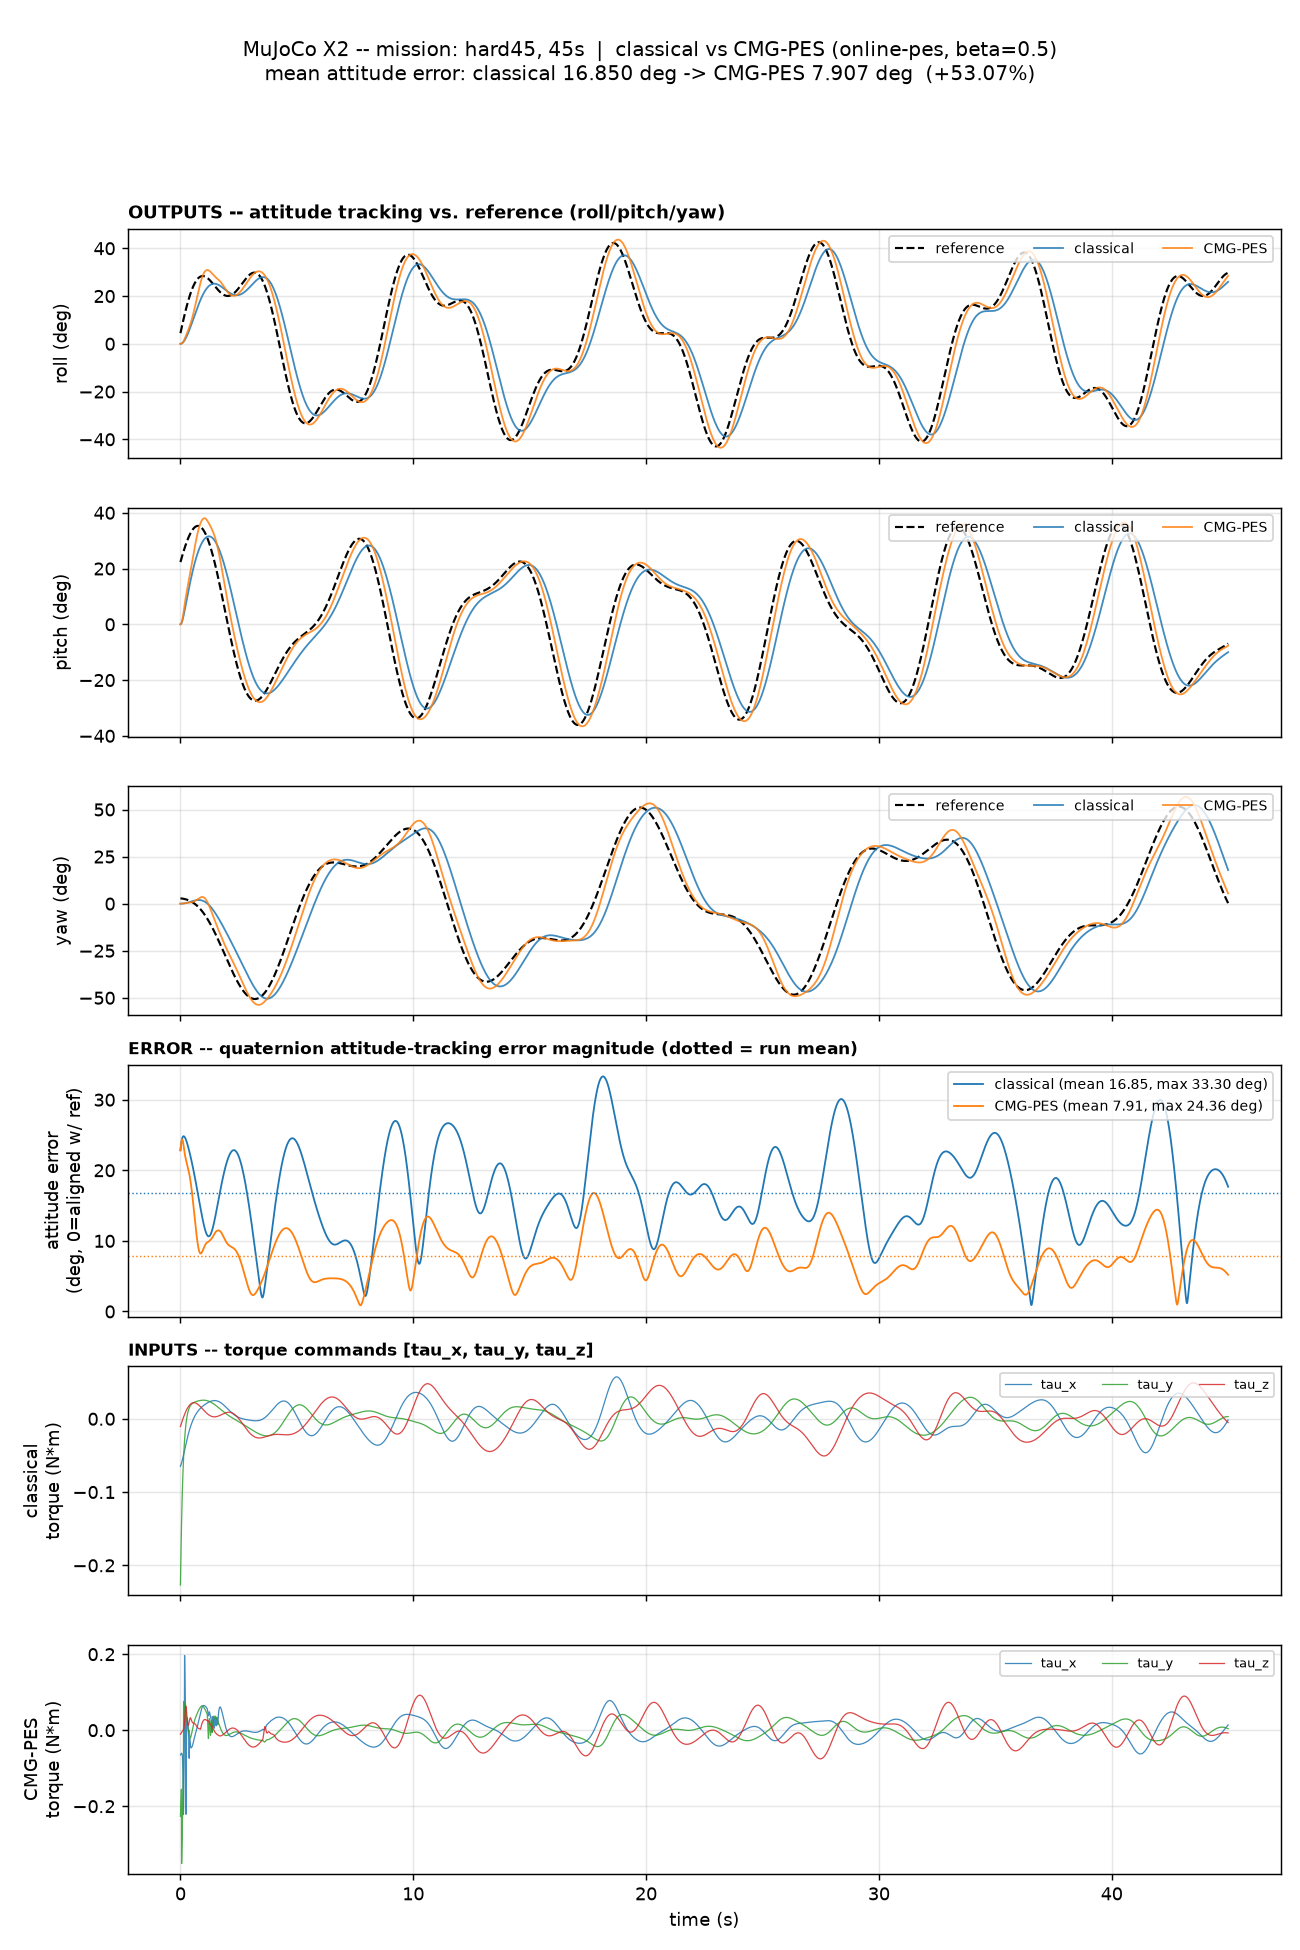
\includegraphics[width=\linewidth]{X2/Hard45/x2_hard45_classical_vs_cmg}
\caption{X2 Hard45: classical baseline vs. CMG--PES residual control.}
\label{fig:tracking}
\end{figure}

\begin{figure}[t]
\centering
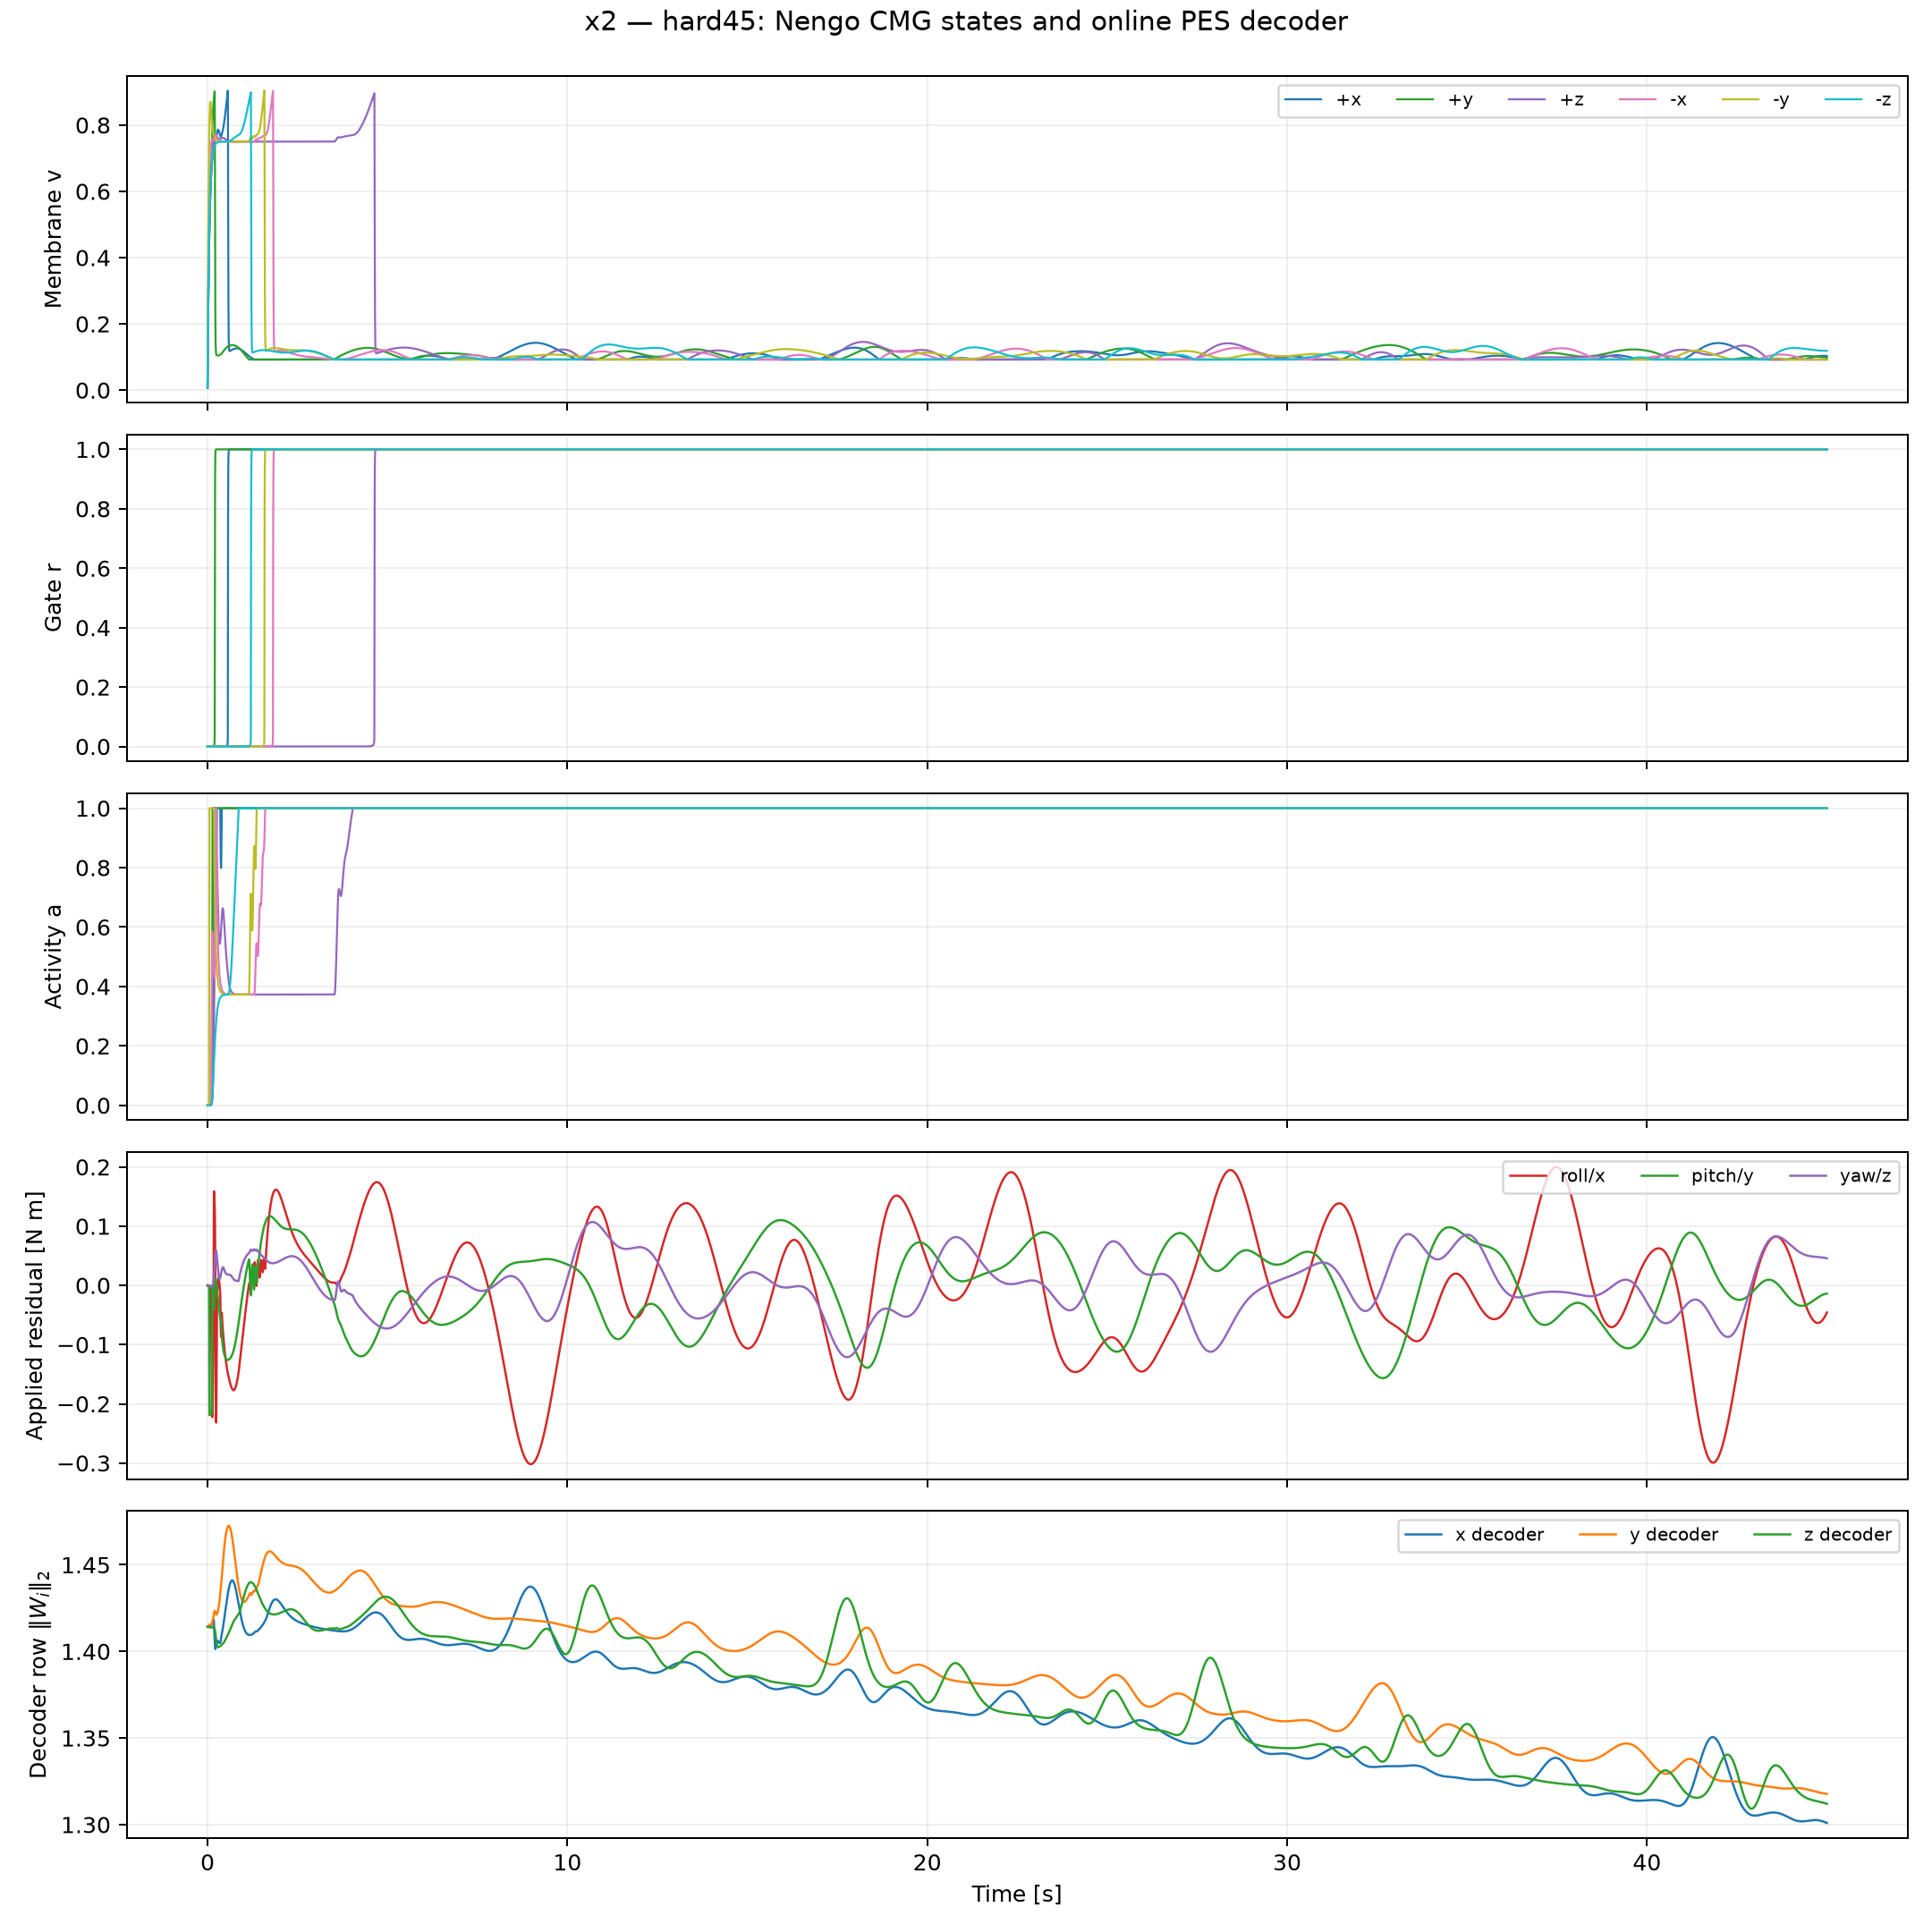
\includegraphics[width=\linewidth]{X2/Hard45/x2_hard45_neurons}
\caption{X2 Hard45: neural activity for the CMG residual controller.}
\label{fig:hard45_neurons}
\end{figure}

\begin{figure}[t]
\centering
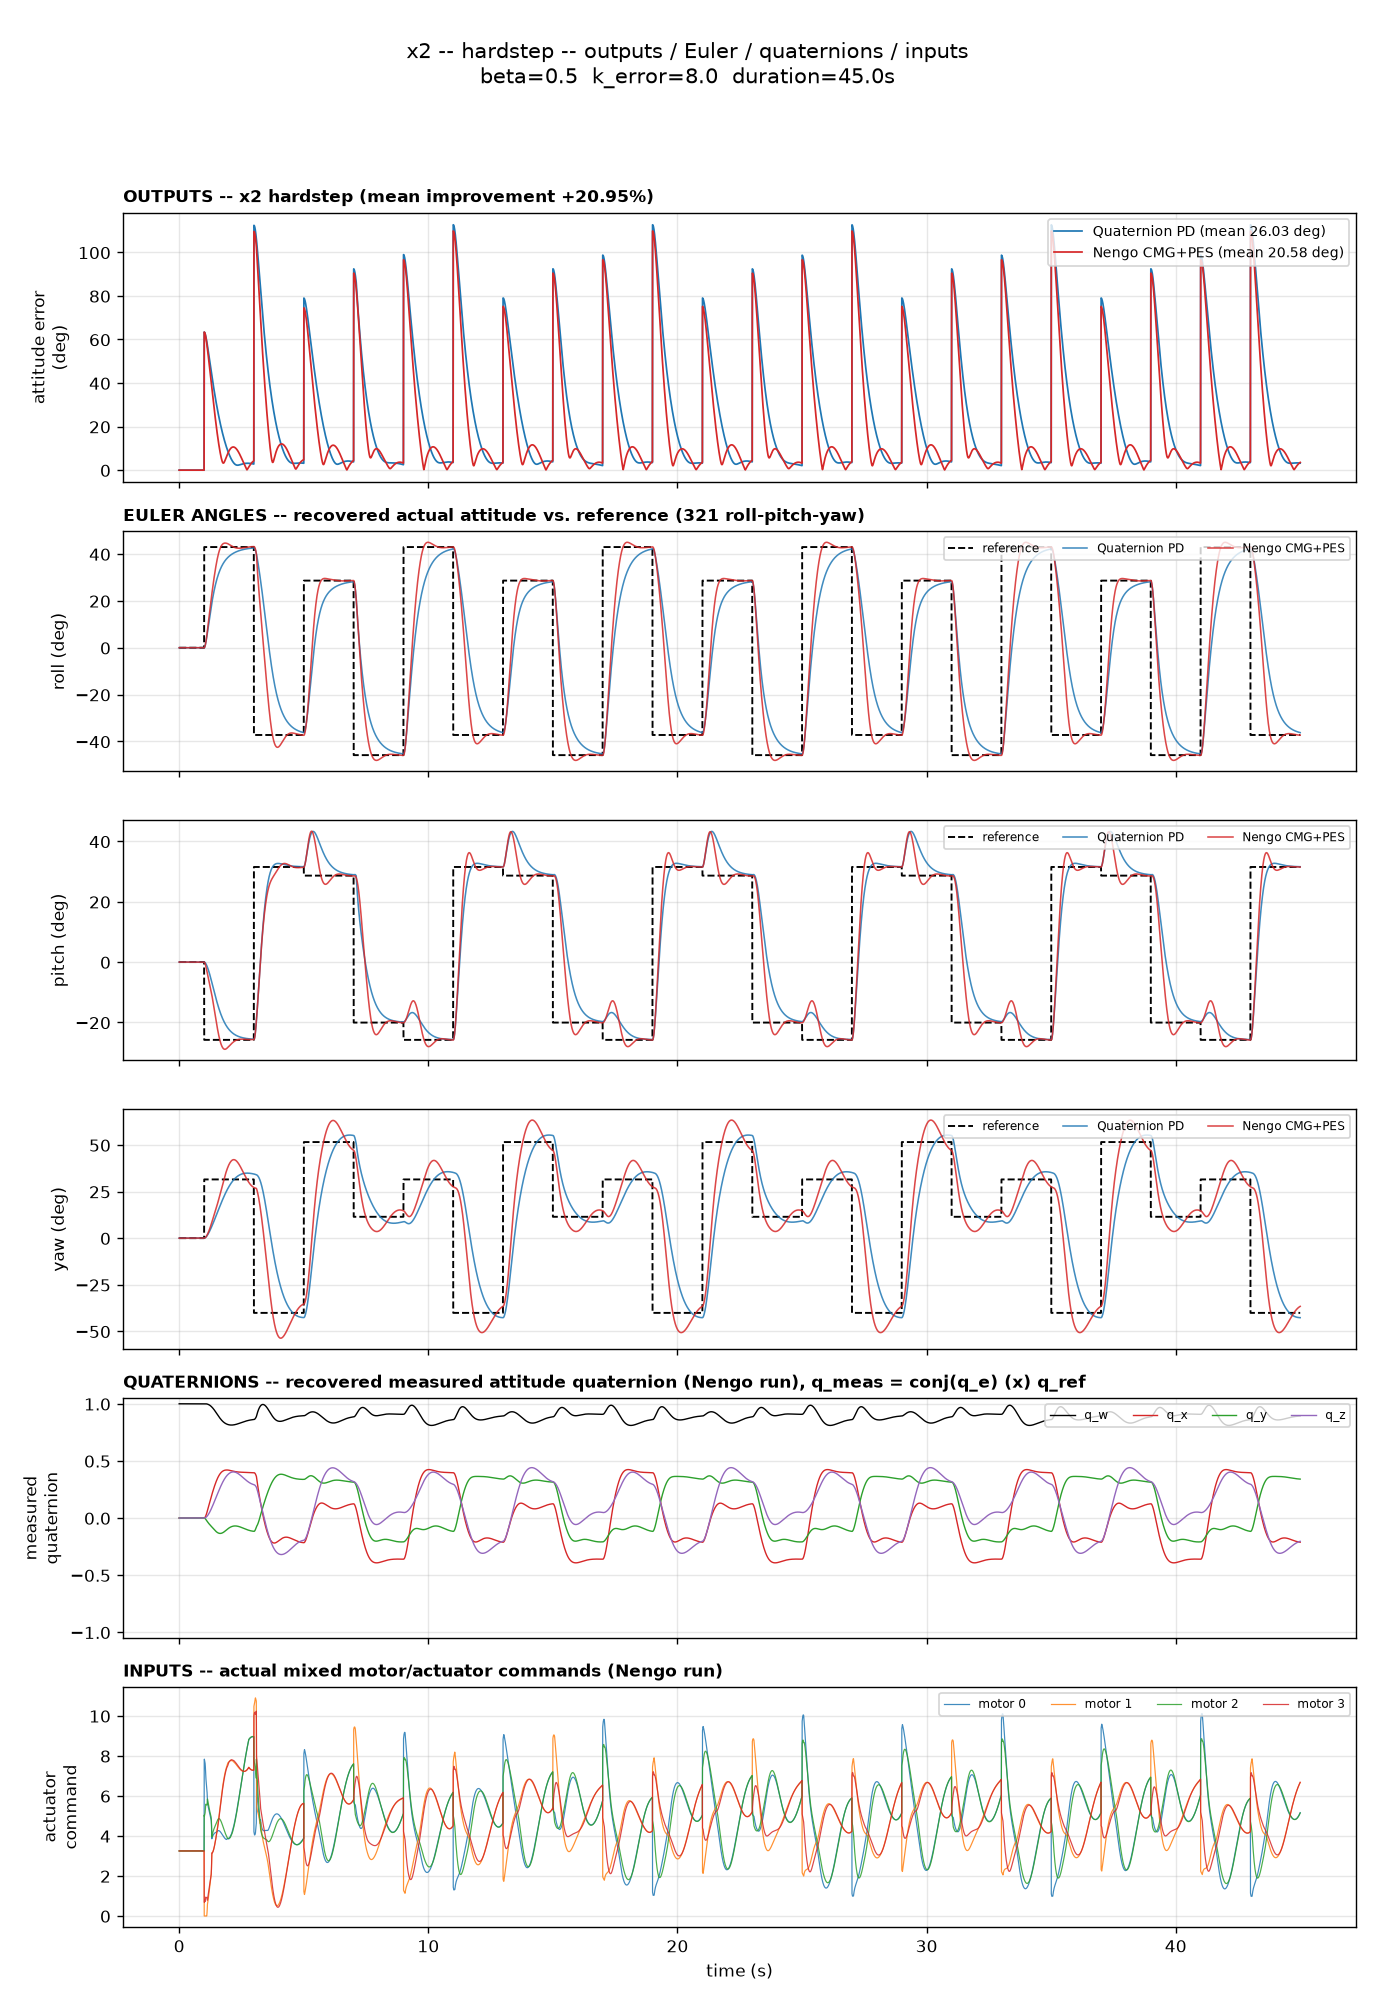
\includegraphics[width=\linewidth]{X2/Hardstep/x2_hardstep_attitude}
\caption{X2 Hardstep: attitude tracking time series (hard step reference).}
\label{fig:hardstep_attitude}
\end{figure}

\begin{figure}[t]
\centering
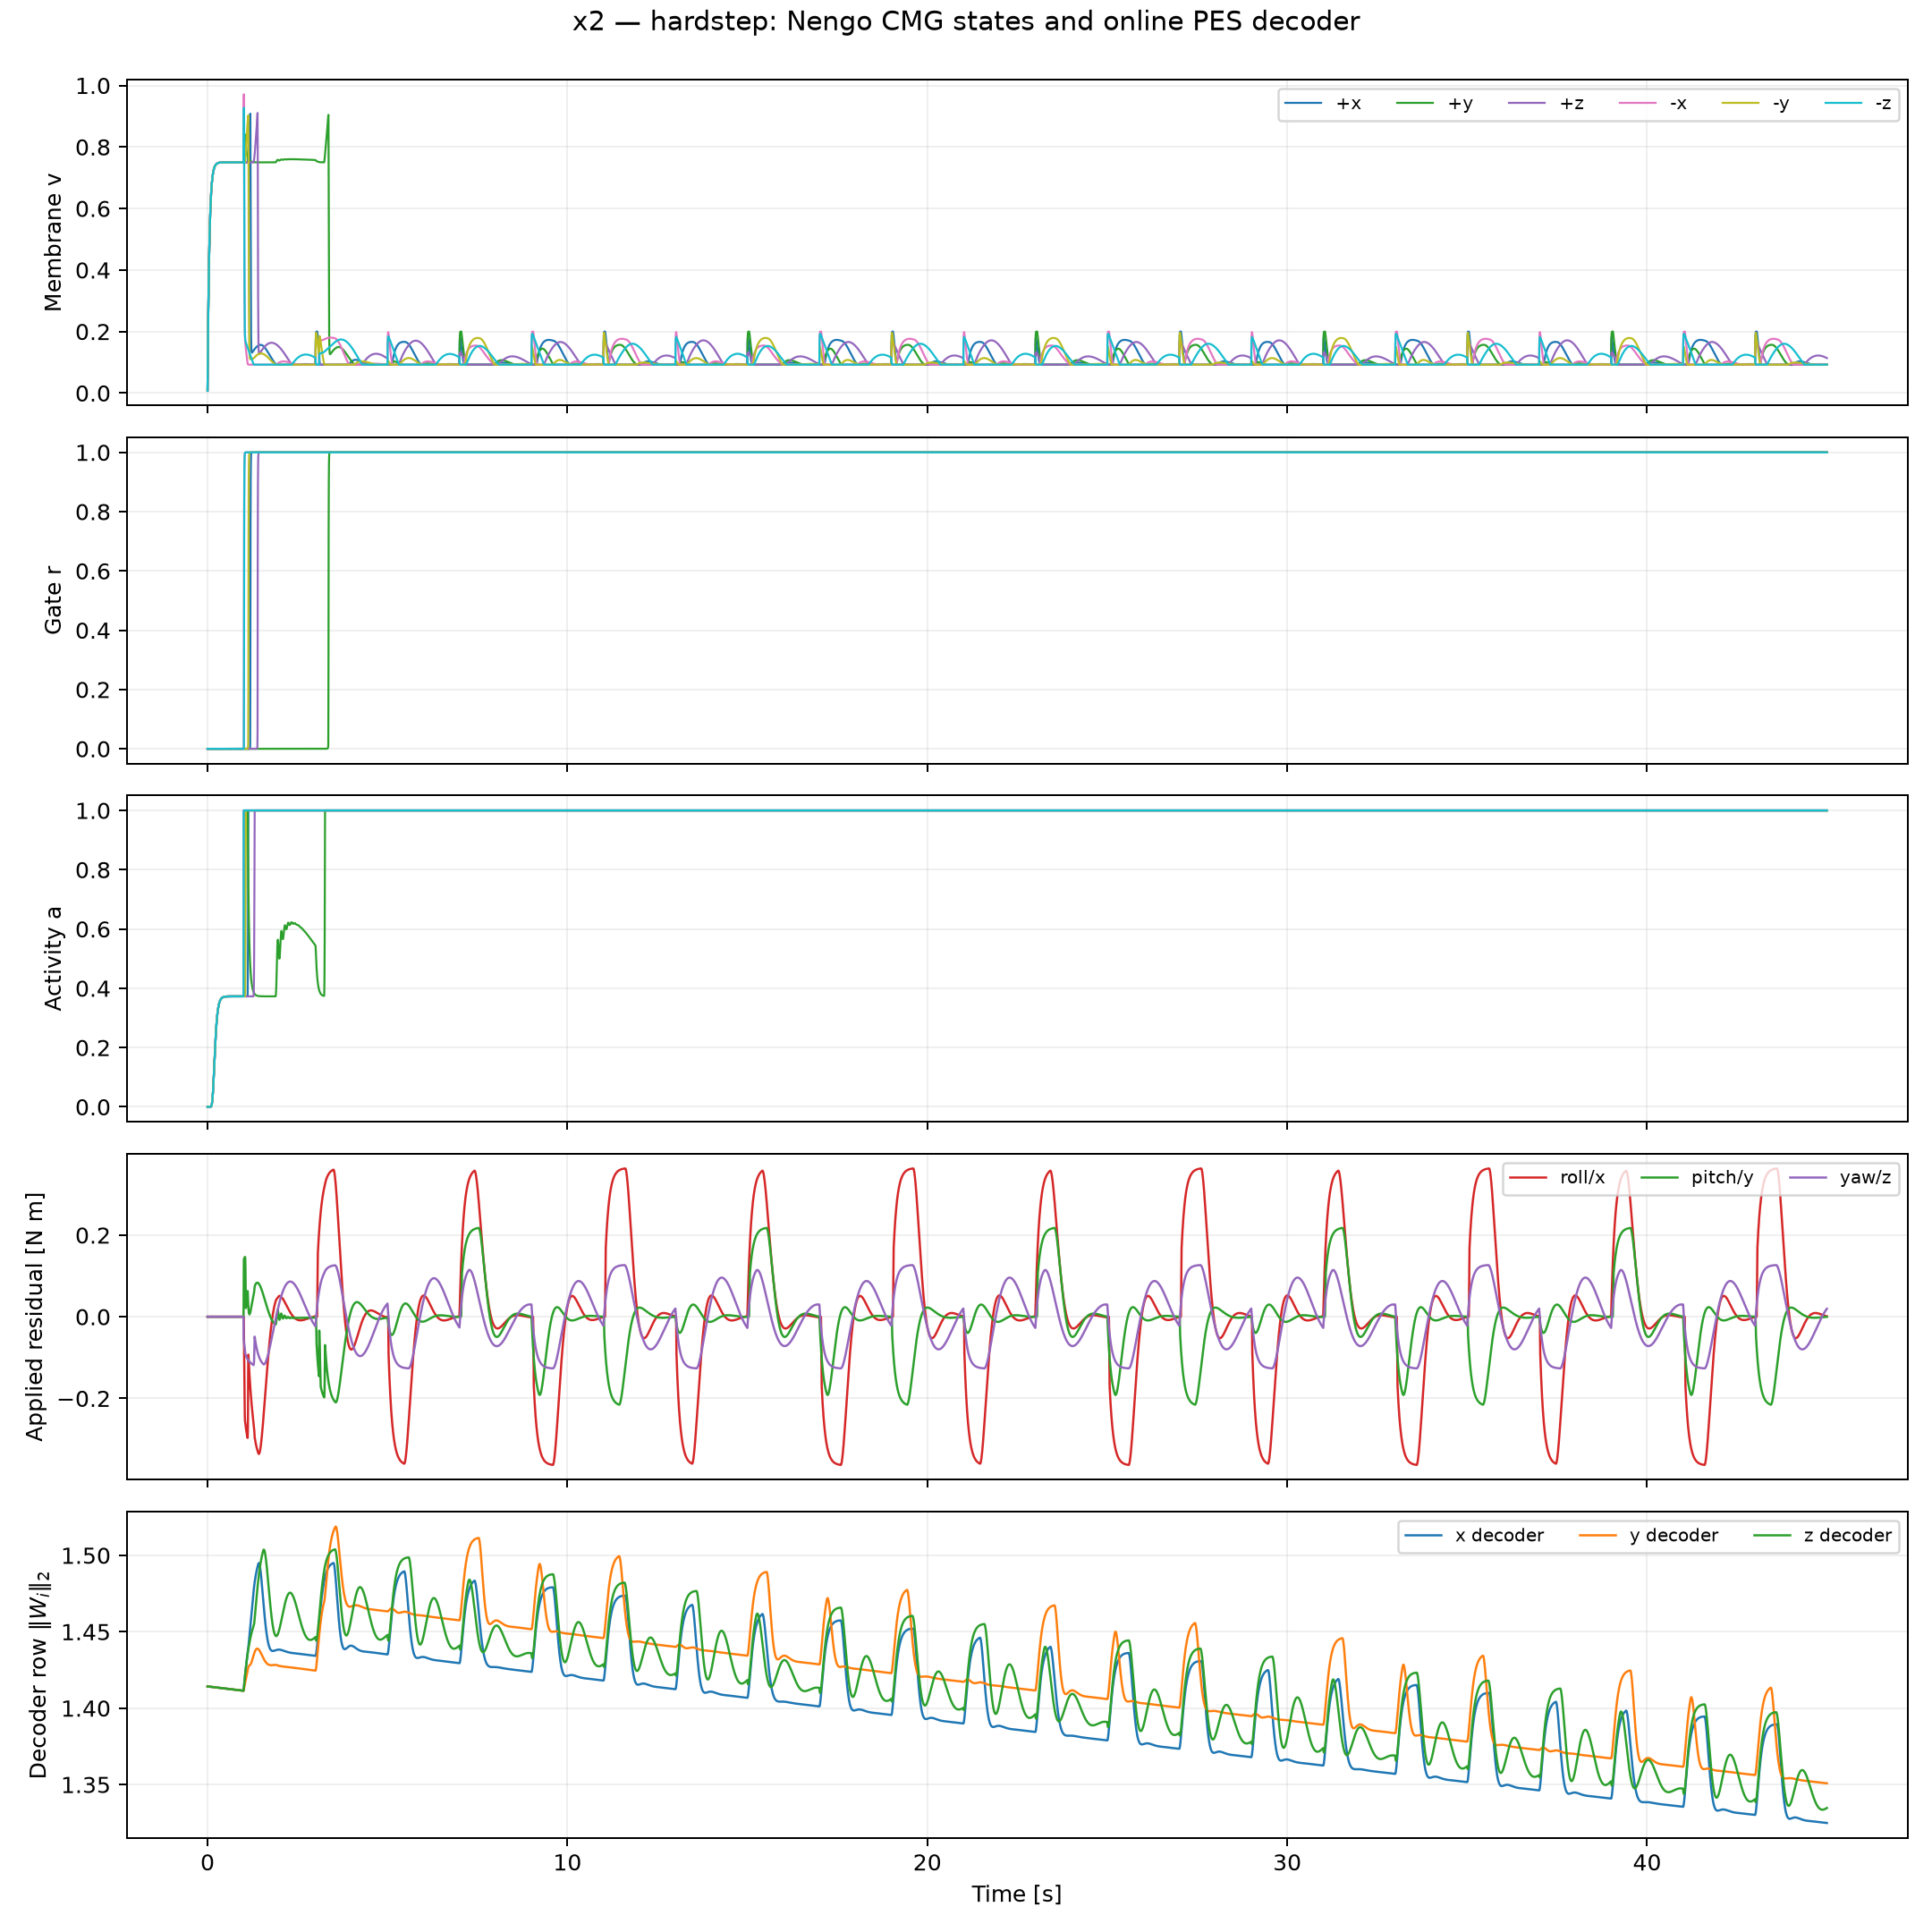
\includegraphics[width=\linewidth]{X2/Hardstep/x2_hardstep_neurons}
\caption{X2 Hardstep: neural activity for the CMG residual controller.}
\label{fig:hardstep_neurons}
\end{figure}

\subsection{What Is Learning?}
Fixed-decoder residuals already improve some missions: in the audited direct
X2 runs their mean reductions range from about 0.12\% to 10.27\%; the
corresponding CF2-design range is 0.06\% to 6.80\%. Thus it is inaccurate
to say that fixing the decoder removes \emph{all} improvement. PES produces
the much larger 17.3--60.6\% primary reductions. Separately, toggling
$\chi$ with the decoder mode held fixed is numerically indistinguishable
under the tested settings. This identifies decoder adaptation as the
principal tested lever, not a universal claim that conductance never matters.

Because $a_j=\clip(10^5r_j,0,1)$, decoder activity saturates already at
$r_j=10^{-5}$. Tiny but nonzero gates can therefore yield order-one
activity while $c_j\propto r_j^2$ remains small. This is a plausible
mechanistic explanation for the observed conductance insensitivity, not
a claim that every gate remains $O(10^{-6})$ at every instant. A calibrated
gate-gain sweep and gate/membrane readout ablation are needed to determine
whether CMG offers benefits beyond a simpler dynamical basis.

\begin{figure}[t]
\centering
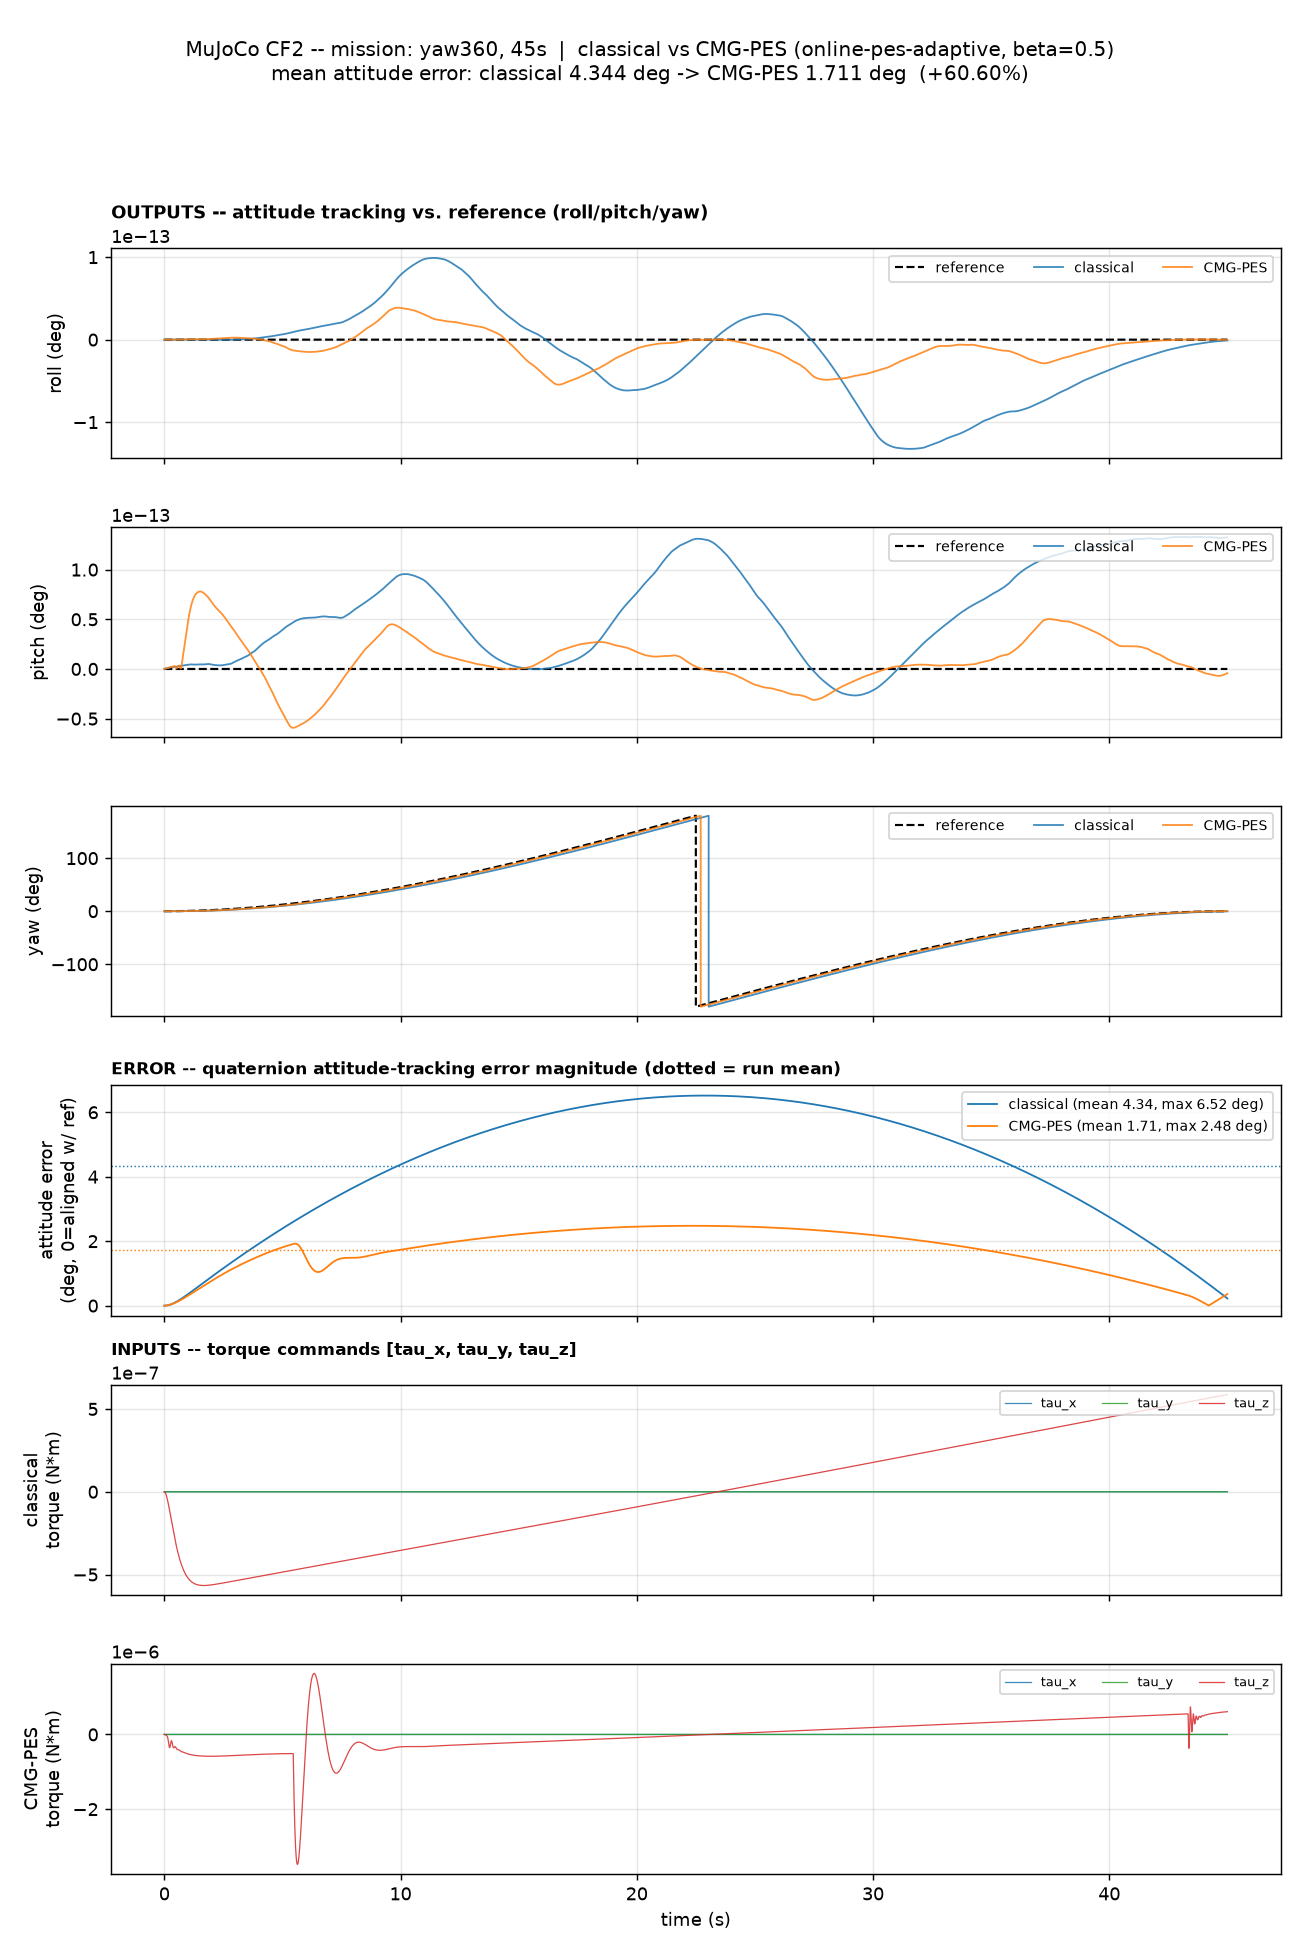
\includegraphics[width=\linewidth]{CF2/Yaw360/cf2_yaw360_classical_vs_cmg}
\caption{CF2 Yaw360: classical baseline vs. CMG--PES residual control.}
\label{fig:states}
\end{figure}

\begin{figure}[t]
\centering
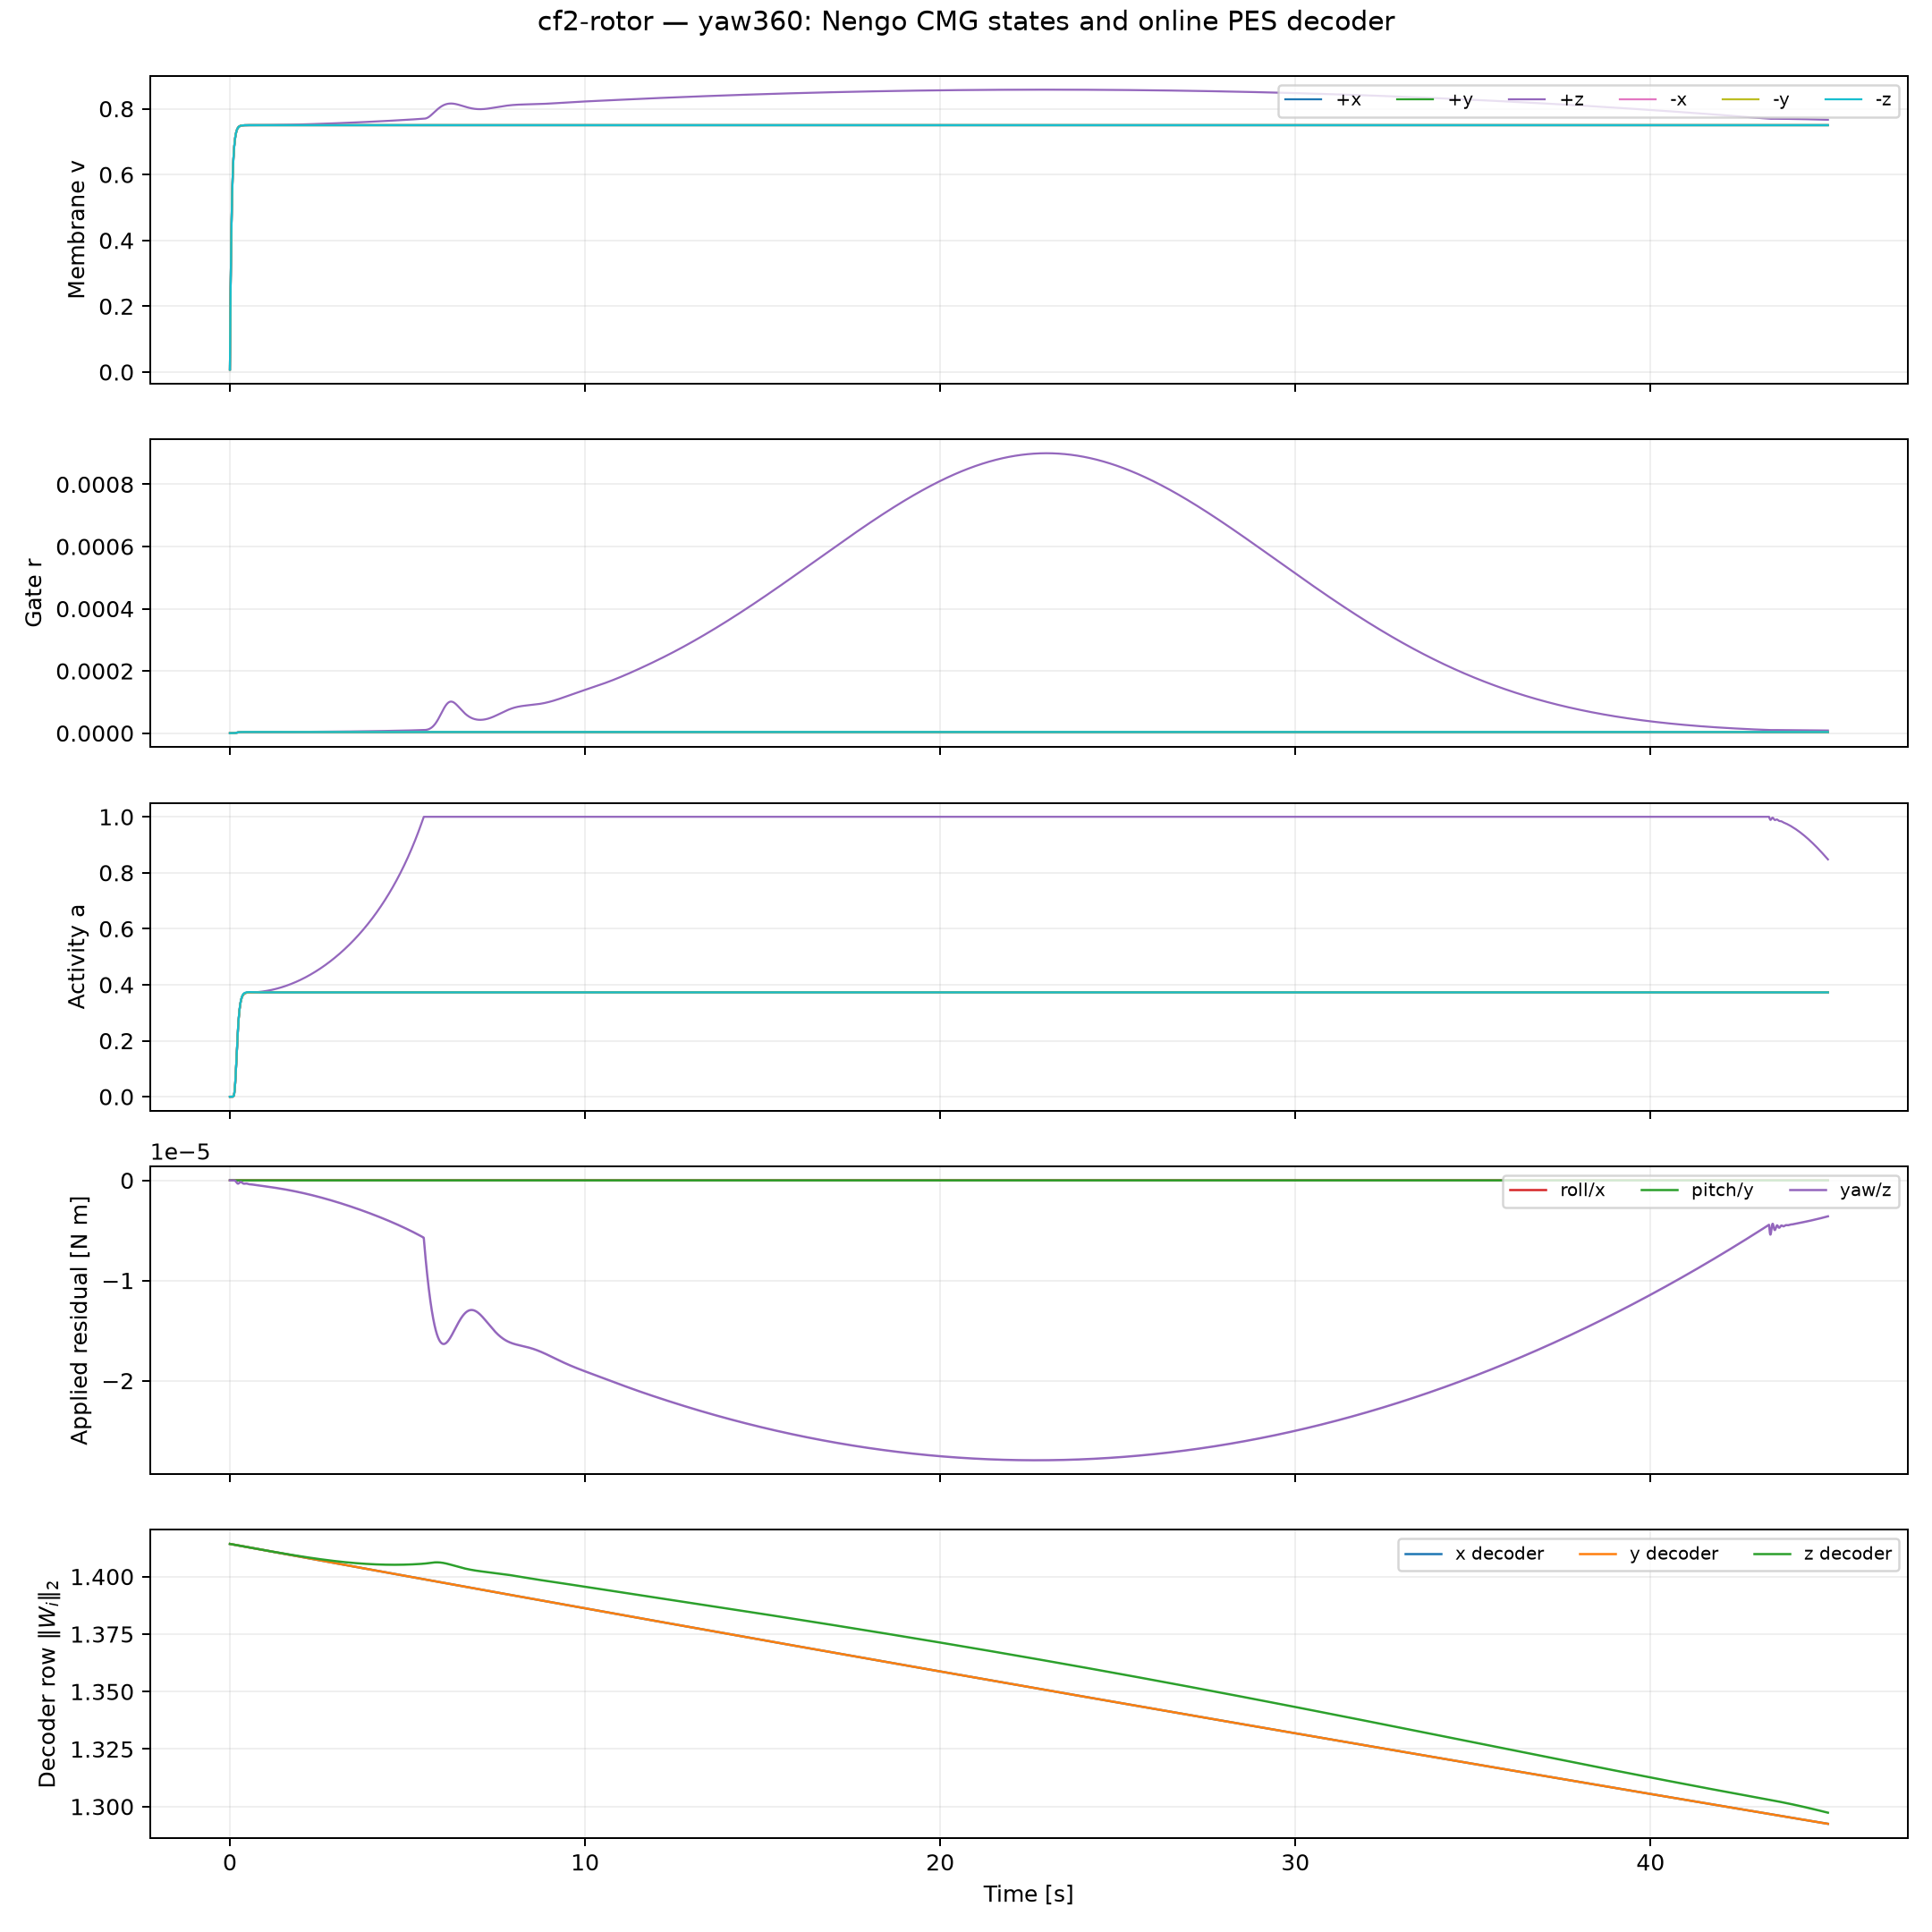
\includegraphics[width=\linewidth]{CF2/Yaw360/cf2-rotor_yaw360_neurons}
\caption{CF2 Yaw360: neural activity for the CMG residual controller.}
\label{fig:cf2_yaw360_neurons}
\end{figure}

Figure~\ref{fig:states} distinguishes the membrane, raw gate, and clipped
activity using the same recorded trajectory rather than equating them.

\subsection{Neuron-Family Comparison}
The Nengo benchmark contains two models, five missions, and eleven
controllers: PD and fixed/PES variants of CMG, LIF, ALIF, Izhikevich
\cite{izhikevich2003}, and LIFRate. All use the same residual/allocator
path, with model-specific native activity and filtering. Some
Izhikevich--PES cells outperform CMG--PES on mean tracking error. The audit
reports an approximate average normalized residual RMS of 0.37 for
Izhikevich--PES versus 0.12 for CMG--PES, alongside more decoder movement.
Equal output caps do not imply equal realized correction effort.
Very sparse LIF/ALIF activity in some tested cells is an operating-point
limitation, not evidence that those neuron families cannot learn.
Accordingly, the supported conclusion is a tracking--effort tradeoff, not
universal CMG superiority or a proven causal effect of spiking.

\section{Annealed Learning: Verified Precursor Evidence}
\label{sec:legacy}
The verified AAT results use the precursor \emph{blend} law
$(1-\beta)\bm u_0+\beta\bm\ell\odot\bm s$ at $\beta=0.5$, with ideal
external-wrench injection and a classical horizontal stabilizer. Its CF2
torque limits also differ from the rotor-design campaign. Therefore these
results are a within-precursor learning-configuration comparison, not
additional rotor-feasible validation of \eqref{eq:residual}.

\begin{table}[t]
\caption{Traceable precursor summaries: mean quaternion-angle error [rad],
$45$ s, $h=0.5$ ms, one run per configuration. AAT corresponds to archived
\texttt{eprop\_anneal}. These results must not be pooled with
Table~\ref{tab:mujoco}.}
\label{tab:aat}\centering\small
\begin{tabular}{llrrr}
\toprule
Model&Mission&PD&PES&AAT\\\midrule
X2&Hard45&.294079&.122051&.127526\\
CF2&Hard45&.285448&.035549&.035445\\
CF2&Hardstep&.661866&1.757814&2.079473\\\bottomrule
\end{tabular}
\end{table}
On Hard45, AAT is slightly better than PES for CF2 and worse for X2.
Both learned configurations severely degrade CF2 Hardstep tracking relative
to that precursor baseline. Since quaternion angle is bounded by $\pi$,
these values indicate a loss of tracking, not mathematical divergence of
the angle or decoder weights. The archived Hardstep saturation field is
zero and the actuation path is ideal wrench; these files do not establish
rotor-allocation saturation as the cause.

The comparison changes eligibility smoothing and learning-rate schedule
together, and the canonical experiment additionally changes residual law
and actuator interface. It therefore does not isolate which change avoids
the precursor failure. At fixed $\beta=0.5$, the blend retains a known
baseline coefficient of $0.5$, not an arbitrarily vanishing coefficient.
The additive law removes this explicit attenuation but cannot by itself
guarantee stability or eliminate adverse step responses. An additive-versus-
blend factorial study with matched actuation, teacher, and learning rate
is the appropriate next test.

\section{Selected Preliminary Physical Tests}
\label{sec:hover}
Before the present manuscript synthesis, CMG--PES was tested on the Quanser
3DOF Hover. These are preliminary supporting tests, not free-flight
validation of either MuJoCo airframe. The rig uses torque-to-motor-voltage
allocation, a 200-Hz Q8 loop, and ten 0.5-ms Nengo substeps per hardware
sample. The representative Roll configuration uses $\beta=0.2$, a 0.2-V
per-motor residual cap, a 1 V/s residual slew limit, $\eta=2\times10^{-4}$,
$k_e=2$, and $k_\omega^*=0$.

Roll is the strongest replicated result: over three matched 8-s pairs, the
recorded mean error is $5.4405\pm0.0648^\circ$ (PD) versus
$5.2960\pm0.0428^\circ$ (CMG--PES), i.e., a paired mean reduction of
$2.65\%\pm1.08\%$ (sample SD, not a confidence interval). These archived
values use the mean norm of the wrapped yaw/pitch/roll error vector (not
$\bar\theta_q$) and are not pooled with the MuJoCo table.

Selected later single pairs show mean-error reductions of 0.55\% (Hard45)
and 0.95\% (scaled, transition-smoothed Hardstep) while worsening peak
errors. Other profiles regress, and no full-scale yaw360 pair was validated.
Thus hardware results support execution feasibility and a small repeated Roll
benefit, but do not explain the simulation-to-hardware discrepancy.

\section{Discussion and Conclusion}
We combine paired continuous CMG dynamics, local online decoder adaptation,
and a bounded additive torque correction around a fixed quaternion-PD law.
Across five missions (ten matched 45-s cases), mean attitude error decreases
by 17.3--60.6\% on two modeled platforms with explicit actuator-bound
accounting; Nengo reproduces the direct implementation, and ablations isolate
decoder learning as the dominant effect in the tested regime. AAT provides a
well-defined alternative memory/schedule mechanism, but its verified results
remain precursor evidence rather than a cross-mission advantage.

Bounded commands, internal states, and projected weights are implementation
properties, not stability/safety proofs. Establishing ISS/Lyapunov results
would require baseline robustness assumptions and bounds on the \emph{realized}
post-allocation perturbation; small voltage caps alone do not quantify
achievable improvement. Follow-up work includes matched-rate AAT/PES
comparisons, equal-effort neuron/readout ablations, stochastic disturbance
trials, frozen-weight held-out tests, repeated hardware perturbations, and
neuromorphic-device energy/latency measurements.

% Finalize human authors, affiliations, funding, and any required tool-use
% disclosure before submission. No invented author identities are supplied.
\bibliographystyle{IEEEtran}
\bibliography{references}
\end{document}
